\documentclass[10pt,twocolumn,letterpaper]{article}

\usepackage{comment}
\usepackage{kotex}
\usepackage{cvpr}
\usepackage{times}
\usepackage{epsfig}
\usepackage{graphicx}
\usepackage{amsmath}
\usepackage{amssymb}
\usepackage{nicefrac}
\usepackage{mathtools}
\usepackage{adjustbox}


\usepackage{caption}
\usepackage{tikz}
\usepackage{pgfplots}
\usetikzlibrary{spy,calc}
\usepackage{array}
\newcolumntype{x}[1]{>{\centering\arraybackslash\hspace{0pt}}p{#1}}
%%%
\newif\ifblackandwhitecycle
\gdef\patternnumber{0}

\pgfkeys{/tikz/.cd,
zoombox paths/.style={
    draw=orange,
    very thick
},
black and white/.is choice,
black and white/.default=static,
black and white/static/.style={
    draw=white,
    zoombox paths/.append style={
        draw=white,
        postaction={
            draw=black,
            loosely dashed
        }
    }
},
black and white/static/.code={
    \gdef\patternnumber{1}
},
black and white/cycle/.code={
    \blackandwhitecycletrue
    \gdef\patternnumber{1}
},
black and white pattern/.is choice,
black and white pattern/0/.style={},
black and white pattern/1/.style={
    draw=white,
    postaction={
        draw=black,
        dash pattern=on 2pt off 2pt
    }
},
black and white pattern/2/.style={
    draw=white,
    postaction={
        draw=black,
        dash pattern=on 4pt off 4pt
    }
},
black and white pattern/3/.style={
    draw=white,
    postaction={
        draw=black,
        dash pattern=on 4pt off 4pt on 1pt off 4pt
    }
},
black and white pattern/4/.style={
    draw=white,
    postaction={
        draw=black,
        dash pattern=on 4pt off 2pt on 2 pt off 2pt on 2 pt off 2pt
    }
},
zoomboxarray inner gap/.initial=5pt,
zoomboxarray columns/.initial=2,
zoomboxarray rows/.initial=2,
subfigurename/.initial={},
figurename/.initial={zoombox},
zoomboxarray/.style={
    execute at begin picture={
        \begin{scope}
            [
            spy using outlines={%
                zoombox paths,
                width=\imagewidth / \pgfkeysvalueof{/tikz/zoomboxarray columns} - (\pgfkeysvalueof{/tikz/zoomboxarray columns} - 1) / \pgfkeysvalueof{/tikz/zoomboxarray columns} * \pgfkeysvalueof{/tikz/zoomboxarray inner gap} -\pgflinewidth,
                height=\imageheight / \pgfkeysvalueof{/tikz/zoomboxarray rows} - (\pgfkeysvalueof{/tikz/zoomboxarray rows} - 1) / \pgfkeysvalueof{/tikz/zoomboxarray rows} * \pgfkeysvalueof{/tikz/zoomboxarray inner gap}-\pgflinewidth,
                magnification=3,
                every spy on node/.style={
                    zoombox paths
                },
                every spy in node/.style={
                    zoombox paths
                }
            }
            ]
    },
    execute at end picture={
        \end{scope}
%\node at (image.north) [anchor=north,inner sep=0pt] {\subcaptionbox{\label{\pgfkeysvalueof{/tikz/figurename}-image}}{\phantomimage}};
%\node at (zoomboxes container.north) [anchor=north,inner sep=0pt] {\subcaptionbox{\label{\pgfkeysvalueof{/tikz/figurename}-zoom}}{\phantomimage}};
\gdef\patternnumber{0}
},
spymargin/.initial=0.5em,
zoomboxes xshift/.initial=1,
zoomboxes right/.code=\pgfkeys{/tikz/zoomboxes xshift=1},
zoomboxes left/.code=\pgfkeys{/tikz/zoomboxes xshift=-1},
zoomboxes yshift/.initial=0,
zoomboxes above/.code={
\pgfkeys{/tikz/zoomboxes yshift=1},
\pgfkeys{/tikz/zoomboxes xshift=0}
},
zoomboxes below/.code={
\pgfkeys{/tikz/zoomboxes yshift=-1},
\pgfkeys{/tikz/zoomboxes xshift=0}
},
caption margin/.initial=0.4ex,
},
adjust caption spacing/.code={},
image container/.style={
inner sep=0pt,
at=(image.north),
anchor=north,
adjust caption spacing
},
zoomboxes container/.style={
inner sep=0pt,
at=(image.north),
anchor=north,
name=zoomboxes container,
xshift=\pgfkeysvalueof{/tikz/zoomboxes xshift}*(\imagewidth+\pgfkeysvalueof{/tikz/spymargin}),
yshift=\pgfkeysvalueof{/tikz/zoomboxes yshift}*(\imageheight+\pgfkeysvalueof{/tikz/spymargin}+\pgfkeysvalueof{/tikz/caption margin}),
adjust caption spacing
},
calculate dimensions/.code={
\pgfpointdiff{\pgfpointanchor{image}{south west} }{\pgfpointanchor{image}{north east} }
\pgfgetlastxy{\imagewidth}{\imageheight}
\global\let\imagewidth=\imagewidth
\global\let\imageheight=\imageheight
\gdef\columncount{1}
\gdef\rowcount{1}
\gdef\zoomboxcount{1}
},
image node/.style={
inner sep=0pt,
name=image,
anchor=south west,
append after command={
[calculate dimensions]
node [image container,subfigurename=\pgfkeysvalueof{/tikz/figurename}-image] {\phantomimage}
node [zoomboxes container,subfigurename=\pgfkeysvalueof{/tikz/figurename}-zoom] {\phantomimage}
}
},
color code/.style={
zoombox paths/.append style={draw=#1}
},
connect zoomboxes/.style={
spy connection path={\draw[draw=none,zoombox paths] (tikzspyonnode) -- (tikzspyinnode);}
},
help grid code/.code={
\begin{scope}[
x={(image.south east)},
y={(image.north west)},
font=\footnotesize,
help lines,
overlay
]
\foreach \x in {0,1,...,9} {
\draw(\x/10,0) -- (\x/10,1);
\node [anchor=north] at (\x/10,0) {0.\x};
}
\foreach \y in {0,1,...,9} {
\draw(0,\y/10) -- (1,\y/10);                        \node [anchor=east] at (0,\y/10) {0.\y};
}
\end{scope}
},
help grid/.style={
append after command={
[help grid code]
}
},
}

\newcommand\phantomimage{%
\phantom{%
\rule{\imagewidth}{\imageheight}%
}%
}
\newcommand\zoombox[2][]{
\begin{scope}[zoombox paths]
\pgfmathsetmacro\xpos{
(\columncount-1)*(\imagewidth / \pgfkeysvalueof{/tikz/zoomboxarray columns} + \pgfkeysvalueof{/tikz/zoomboxarray inner gap} / \pgfkeysvalueof{/tikz/zoomboxarray columns} ) + \pgflinewidth
}
\pgfmathsetmacro\ypos{
(\rowcount-1)*( \imageheight / \pgfkeysvalueof{/tikz/zoomboxarray rows} + \pgfkeysvalueof{/tikz/zoomboxarray inner gap} / \pgfkeysvalueof{/tikz/zoomboxarray rows} ) + 0.5*\pgflinewidth
}
\edef\dospy{\noexpand\spy [
#1,
zoombox paths/.append style={
black and white pattern=\patternnumber
},
every spy on node/.append style={#1},
x=\imagewidth,
y=\imageheight
] on (#2) in node [anchor=north west] at ($(zoomboxes container.north west)+(\xpos pt,-\ypos pt)$);}
\dospy
\pgfmathtruncatemacro\pgfmathresult{ifthenelse(\columncount==\pgfkeysvalueof{/tikz/zoomboxarray columns},\rowcount+1,\rowcount)}
\global\let\rowcount=\pgfmathresult
\pgfmathtruncatemacro\pgfmathresult{ifthenelse(\columncount==\pgfkeysvalueof{/tikz/zoomboxarray columns},1,\columncount+1)}
\global\let\columncount=\pgfmathresult
\ifblackandwhitecycle
\pgfmathtruncatemacro{\newpatternnumber}{\patternnumber+1}
\global\edef\patternnumber{\newpatternnumber}
\fi
\end{scope}
}

%%%
\usepackage[acronym,shortcuts]{glossaries}
\DeclarePairedDelimiter\ceil{\lceil}{\rceil}
\DeclarePairedDelimiter\floor{\lfloor}{\rfloor}
\newcommand{\Mod}[2]{\text{mod}\left(#1,#2\right)}
\usepackage{setspace}

%
\usepackage[pagebackref=true,breaklinks=true,letterpaper=true,colorlinks,bookmarks=false]{hyperref}

\usepackage{booktabs}

\cvprfinalcopy

\def\cvprPaperID{1948} % *** Enter the CVPR Paper ID here
\def\httilde{\mbox{\tt\raisebox{-.5ex}{\symbol{126}}}}

% Pages are numbered in submission mode, and unnumbered in camera-ready
\ifcvprfinal\pagestyle{empty}\fi

\makeglossaries

\newacronym{SISR}{SISR}{single image super-resolution}
\newacronym{단일 이미지 초해상도화}{단일 이미지 초해상도화}{single image super-resolution}
\newacronym{PSNR}{PSNR}{peak signal-to-noise ratio}
\newacronym{MSE}{MSE}{mean squared error}
\newacronym{평균 제곱 오차}{평균 제곱 오차}{mean squared error}
\newacronym{CNN}{CNN}{convolutional neural network}
\newacronym{합성곱 신경망}{합성곱 신경망}{convolutional neural network}
\newacronym{ESPCN}{ESPCN}{efficient sub-pixel convolutional neural network}
\newacronym{DRCN}{DRCN}{deeply-recursive convolutional network}
\newacronym{ResNet}{ResNet}{residual network}
\newacronym{GAN}{GAN}{generative adversarial network}
\newacronym{LR}{LR}{low-resolution}
\newacronym{저해상도}{저해상도}{low-resolution}
\newacronym{HR}{HR}{high-resolution}
\newacronym{고해상도}{고해상도}{high-resolution}
\newacronym{SR}{SR}{super-resolution}
\newacronym{초해상도화}{초해상도화}{super-resolution}
\newacronym{MOS}{MOS}{mean opinion score}
\newacronym{SSIM}{SSIM}{structural similarity}
\newacronym{PSNR-HVS}{PSNR-HVS}{peak signal-to-noise ratio - human visual system}
\newacronym{MS-SSIM}{MS-SSIM}{multi-scale structural similarity}
\newacronym{SRGAN}{SRGAN}{super-resolution generative adversarial network}

\newcommand{\lrimage}[0]{\mathbf{I}^{LR}}
\newcommand{\hrimage}[0]{\mathbf{I}^{HR}}
\newcommand{\networkoutput}[0]{\mathbf{I}^{SR}}
\newcommand{\convolution}[2]{#1\ast#2}
\newcommand{\nonlinearity}[0]{\phi}
\newcommand{\periodicshufflingoperator}[0]{\mathcal{PS}}
\newcommand{\kor}[1]{#1}
\newcommand{\eng}[1]{}

\usepackage{subcaption}

\hyphenpenalty=1000
\tolerance=1000

\begin{document}

%%%%%%%%% TITLE
%\title{Photo-Realistic Single Image Super-Resolution Using a Generative Adversarial Network}
\title{
\eng{Photo-Realistic Single Image Super-Resolution Using a Generative Adversarial Network}
\kor{생성적 적대 신경망을 이용한 실사 단일 이미지 초해상도화}}

\onehalfspacing
\author{Christian Ledig, Lucas Theis, Ferenc Husz\'{a}r, Jose Caballero, Andrew Cunningham, \\Alejandro Acosta, Andrew Aitken, Alykhan Tejani, Johannes Totz, Zehan Wang, Wenzhe Shi\\
Twitter\\
{\tt\footnotesize \{cledig,ltheis,fhuszar,jcaballero,aacostadiaz,aaitken,atejani,jtotz,zehanw,wshi\}@twitter.com}
}

\maketitle

%%%%%%%%% ABSTRACT
\singlespacing
\begin{abstract}
%Super-resolution aims at predicting or recovering lost information and is thus a highly ill-posed problem with a large set of possible solutions.
\eng{
Despite the breakthroughs in accuracy and speed of single image super-resolution using faster and deeper convolutional neural networks, one central problem remains largely unsolved: how do we recover the finer texture details when we super-resolve at large upscaling factors?
}\kor{
더 빠르고 깊은 합성곱 신경망을 사용하는 단일 이미지 초해상도화 기술에 대한 정확도와 속도의 획기적인 약진에도 불구하고, "큰 해상도 향상 인자를 사용해서 초해상도 이미지를 생성할 때, 어떻게 해야 고품질 질감의 세부 사항을 복구할 수 있는가?"라는 중요한 문제는 해결되지 않았다.
}\eng{
The behavior of optimization-based super-resolution methods is principally driven by the choice of the objective function. Recent work has largely focused on minimizing the mean squared reconstruction error.
}\kor{
최적화 기반 초해상도 방법의 동작은 주로 목적 함수를 선택하는 것에 의해 좌우된다. 최근 연구는 평균 제곱 재구성 오류 최소화하는 것에 크게 초점이 맞춰져 있다.
}\eng{
The resulting estimates have high peak signal-to-noise ratios, but they are often lacking high-frequency details and are perceptually unsatisfying in the sense that they fail to match the fidelity expected at the higher resolution.
}\kor{
추정 결과들은 높은 최대 신호 대 잡음비(PSNR)를 가지지만 보통 고주파 세부 사항이 부족한 경우를 보이고, 이는 높은 해상도에서 기대되는 정확도와 일치하지 않는다는 점에서 지각적으로 불만족스럽다.
}\eng{
In this paper, we present SRGAN, a generative adversarial network (GAN) for image super-resolution (SR).
}\kor{
본 논문에서는 이미지 초해상도화를 위한 생성적 적대 신경망인 SRGAN을 제시한다.
}\eng{
 To our knowledge, it is the first framework capable of inferring photo-realistic natural images for $4\times$ upscaling factors.
}\kor{
 우리가 아는 한, SRGAN은 $4\times$ 해상도 향상 인자로 자연스러운 실사 이미지 추론을 할 수 있는 첫번째 프레임워크이다.
}\eng{
 To achieve this, we propose a perceptual loss function which consists of an adversarial loss and a content loss.
}\kor{
 이를 달성하기 위해서, 적대적 손실(loss)와 내용 손실(loss)로 구성된 지각 손실 함수를 제안한다.
}\eng{
 The adversarial loss pushes our solution to the natural image manifold using a discriminator network that is trained to differentiate between the super-resolved images and original photo-realistic images.
}\kor{
초해상도화 이미지와 원본 실사 이미지를 구별하도록 훈련된 판별기(discriminator) 네트워크를 이용해서 적대적 손실은 해(solution)를 자연 이미지 데이터 공간(manifold)로 밀어넣는다.
}\eng{
 In addition, we use a content loss motivated by perceptual similarity instead of similarity in pixel space.
}\kor{
 추가적으로, 픽셀 공간의 유사성 대신 지각적 유사성으로부터 영감를 받은 내용 손실(content loss)이 사용된다.
}\eng{
 Our deep residual network is able to recover photo-realistic textures from heavily downsampled images on public benchmarks.
}\kor{
본 논문에서 제시하는 심층 잔류 신경망은 공개 벤치마크에서 심하게 다운샘플링된 이미지로부터 실사와 같은 질감을 복구해낼 수 있다.
}\eng{
An extensive mean-opinion-score (MOS) test shows hugely significant gains in perceptual quality using SRGAN.
}\kor{
대규모 평균 의견 점수(mean opinion score) 검사는 SRGAN을 사용할 때 지각 품질이 상당히 크게 향상된 것을 보여준다.
}\eng{
 The MOS scores obtained with SRGAN are closer to those of the original high-resolution images than to those obtained with any state-of-the-art method.
}\kor{
 SRGAN으로부터 얻어진 평균 의견 점수는 어떠한 최첨단 방법으로 얻어진 점수보다도 원본 고해상도 이미지의 점수에 가깝다.
}
\end{abstract}

%%%%%%%%% BODY TEXT
\section{서론}
\eng{
The highly challenging task of estimating a \ac{HR} image from its \ac{LR} counterpart is referred to as \ac{SR}.
}\kor{
\ac{고해상도} 이미지에 대응하는 \ac{저해상도} 이미지로부터 \ac{고해상도} 이미지를 추정하는 상당히 도전적인 작업을 \ac{초해상도화}라고 한다.
}\eng{
\ac{SR} received substantial attention from within the computer vision research community and has a wide range of applications \cite{yang2007spatial,Zou12,Nasrollahi2014}.
}\kor{
\ac{초해상도화}는 컴퓨터 비전 연구 공동체 내에서 상당한 관심을 받았으며, 광범위하게 응용되고 있다 \cite{yang2007spatial,Zou12,Nasrollahi2014}.
}
% includes face recognition in surveillance videos \cite{Zou12}, super-resolution of depth maps \cite{yang2007spatial}, video streaming and medical applications.

\begin{figure}[ht]
\begin{tabular}{cc}
\eng{$4\times$ SRGAN (proposed) & original \\}\kor{$4\times$ SRGAN (제안된) & 원본 \\}
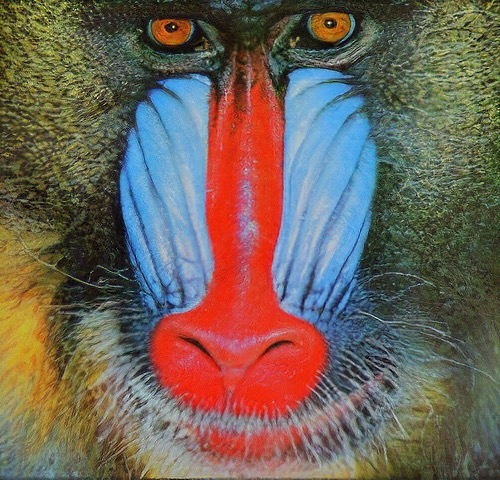
\includegraphics[trim=0 0 0 0, clip, width=1.5in]{images/used/jpg/baboon_SRGAN-VGG54} &
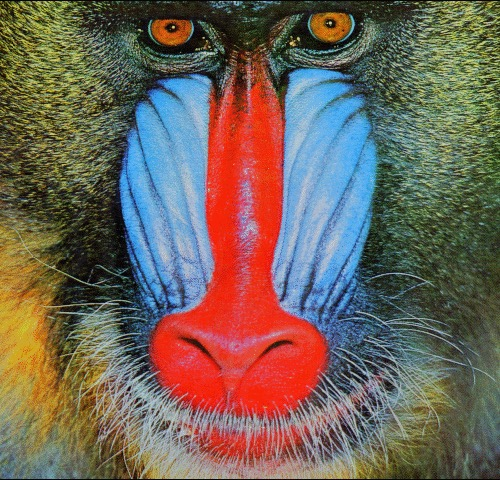
\includegraphics[trim=0 0 0 0, clip, width=1.5in]{images/used/jpg/baboon_HR} \\

\end{tabular}
\caption{
\eng{
Super-resolved image (left) is almost indistinguishable from original (right). [$4\times$ upscaling]
}\kor{
초해상도화된 이미지(좌측)는 원본(우측)과 거의 구분이 불가능하다. [$4\times$ 해상도 향상]
}}
\label{fig:exampleIntroFirst}
\end{figure}

%One major difficulty when estimating the \ac{HR} image is the ambiguity of solutions to the underdetermined \ac{SR} problem.
\eng{
The ill-posed nature of the underdetermined \ac{SR} problem is particularly pronounced for high upscaling factors, for which texture detail in the reconstructed \ac{SR} images is typically absent.
}\kor{
불량 조건인(\ac{저해상도}를 \ac{고해상도}로 복원하는 경우 정답이 1개가 아닌 여러개가 존재하는 것을 불량 조건을 가진다고 함) 미결정 \ac{초해상도화} 문제의 본질은 특히 일반적으로 재구성된 \ac{초해상도화} 이미지의 질감 세부 사항이 없는 높은 해상도 향상 인자에서 두드러진다.
}
%Assumptions about the data have to be made to approximate the \ac{HR} image, such as exploiting image redundancies. % or employing specifically trained feature models.
%
%	Over the last few decades substantial advances have been made in image \ac{SR} \cite{Nasrollahi2014, Yang14benchmark}, with early methods based on interpolation, simple image features (e.g. edges) or statistical image priors.
%	Later example-based methods very successfully detected and exploited patch correspondences within a training database or calculated optimized dictionaries allowing for high-detail data representation. While of good accuracy, the involved optimization procedures for both patch detection and sparse coding are computationally intensive.
%	More advanced methods formulate image-based \ac{SR} as a regression problem that can be tackled for example with Random Forests \cite{schulter2015fast}.
%	The recent rise of \acp{CNN} also had a substantial impact on image \ac{SR} \cite{dong2016image}, not only improving the state of the art with respect to accuracy but also computational speed, enabling real-time \ac{SR} for 2D video frames \cite{Shi2016ESPCN}.
%
\begin{figure*}[ht]
\begin{tabular}{cccc}
\eng{bicubic &  SRResNet  & SRGAN & original}\kor{쌍삼차 보간(bicubic) &  SRResNet  & SRGAN & 원본}\\
(21.59dB/0.6423) &   (23.53dB/0.7832) & (21.15dB/0.6868) & \\

\includegraphics[trim=0pt 0pt 0pt 0pt, clip, width=1.55in]{images/used/jpg/comic_SRF_4_bicubic} &
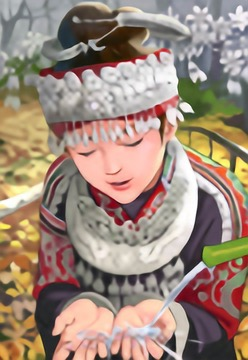
\includegraphics[trim=0pt 0pt 0pt 0pt, clip, width=1.55in]{images/used/jpg/comic_SRResNet-MSE} &
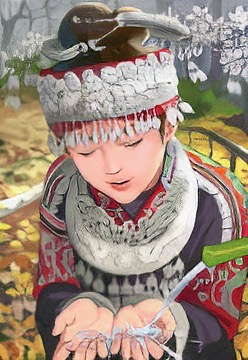
\includegraphics[trim=0pt 0pt 0pt 0pt, clip, width=1.55in]{images/used/jpg/comic_SRGAN-VGG54} &
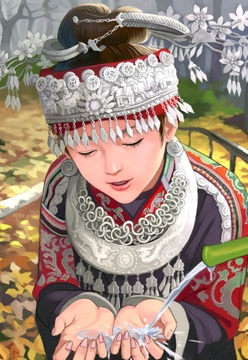
\includegraphics[trim=0pt 0pt 0pt 0pt, clip, width=1.55in]{images/used/jpg/comic_HR.jpg} \\
\end{tabular}
\caption{
\eng{
From left to right: bicubic interpolation, deep residual network optimized for MSE, deep residual generative adversarial network optimized for a loss more sensitive to human perception, original HR image. Corresponding PSNR and SSIM are shown in brackets. [$4\times$ upscaling]
}\kor{
왼쪽에서 오른쪽 순으로: 쌍삼차 보간(bicubic), MSE로 최적화된 심층 잔류 신경망, 원본 고해상도 이미지에 대해서 조금 더 사람의 지각에 민감한 손실로 최적화된 심층 잔류 생성적 적대 신경망. PSNR과 SSIM은 괄호 안에 표시된다. [$4\times$ 해상도 향상]
}
}
\label{fig:exampleIntro}
\end{figure*}
%
\eng{
The optimization target of supervised \ac{SR} algorithms is commonly the minimization of the \ac{MSE} between the recovered \ac{HR} image and the ground truth.
}\kor{
지도 \ac{초해상도화} 알고리듬의 최적화 목표는 보통 \ac{고해상도} 이미지와 정답 사이의 \ac{MSE}를 최소화하는 것이다.
}\eng{
 This is convenient as minimizing \ac{MSE} also maximizes the \ac{PSNR}, which is a common measure used to evaluate and compare \ac{SR} algorithms \cite{Yang14benchmark}.
}\kor{
\ac{MSE}를 최적화하는 것은 \ac{초해상도화} 알고리듬을 평가하고 비교하는데 일반적으로 사용되는 \ac{PSNR}을 최대화하기 때문에 편리하다.\cite{Yang14benchmark}
}
\eng{
However, the ability of MSE (and PSNR) to capture perceptually relevant differences, such as high texture detail, is very limited as they are defined based on pixel-wise image differences \cite{Wang2003,Wang2004,Gupta2011}.
}\kor{
하지만, MSE(그리고 PSNR)의 높은 질감 세부 정보와 같은 지각적으로 관련된 차이를 포착하는 능력은 픽셀 단위의 이미지 차이\cite{Wang2003,Wang2004,Gupta2011}를 기반으로 정의되었기 때문에 매우 제한적이다.
}\eng{
 This is illustrated in \figurename~\ref{fig:exampleIntro}, where highest PSNR does not necessarily reflect the perceptually better \ac{SR} result.
}\kor{
 이것은 높은 PSNR이 필연적으로 지각적으로 더 높은 \ac{초해상도화} 결과를 반영하지 않는 경우인 \figurename~\ref{fig:exampleIntro}에서 보여진다.
}\eng{
 The perceptual difference between the super-resolved and original image means that the recovered image is not photo-realistic as defined by Ferwerda \cite{Ferwerda2003}.
}\kor{
초해상도 (생성물)과 원본 이미지 사이의 지각적 차이는 복원된 이미지는 Ferwerda \cite{Ferwerda2003}에서 정의된 것처럼 실사적이지 않다는 것이다.
}


\eng{
In this work we propose a \ac{SRGAN} for which we employ a deep \ac{ResNet} with skip-connection and diverge from \ac{MSE} as the sole optimization target.
}\kor{
본 논문에서는 건너뛴 연결(skip-connection)을 사용하고 단일 최적화 목표로부터 \ac{MSE}를 분리한 심층 \ac{ResNet}을 이용한 \ac{SRGAN}을 제안한다.
}\eng{
 Different from previous works, we define a novel perceptual loss using high-level feature maps of the VGG network \cite{simonyan2014very,Johnson16PercepLoss,bruna2016super} combined with a discriminator that encourages solutions perceptually hard to distinguish from the \ac{HR} reference images.
}\kor{
 이전 연구와 달리, \ac{고해상도} 참조 이미지와 지각적으로 구분하기 어려운 해들(solutions)을 부추기는 판별기(discriminator)와 결합한 VGG 네트워크 \cite{simonyan2014very,Johnson16PercepLoss,bruna2016super}의 고수준 특징 맵을 사용해서 새로운 지각 손실을 정의한다.
}
\eng{
An example photo-realistic image that was super-resolved with a $4\times$ upscaling factor is shown in \figurename~\ref{fig:exampleIntroFirst}.
}\kor{
$4\times$ 해상도 향상 인자로 초해상도화한 예제 실사 이미지는 \figurename~\ref{fig:exampleIntroFirst}에서 보여진다.
}

\subsection{관련 연구}
\subsubsection{이미지 초해상도화}
%There is a vast amount of literature and research that focuses on image \ac{SR}.
\eng{
Recent overview articles on image \ac{SR} include Nasrollahi and Moeslund \cite{Nasrollahi2014} or Yang et al. \cite{Yang14benchmark}.
}\kor{
최근 이미지 \ac{초해상도화} 분야의 개요적 기사에는 Nasrollahi와 Moeslund \cite{Nasrollahi2014} 또는 Yang 외. 가 있다.
}\eng{
Here we will focus on \ac{SISR} and will not further discuss approaches that recover \ac{HR} images from multiple images \cite{Borman1998aSurvey,Farsiu2004}.
}\kor{
본 논문에서는 \ac{단일 이미지 초해상도화}에 초점을 맞추고, 고해상도 \ac{고해상도} 이미지들을 여러 이미지로부터 복원하는 \cite{Borman1998aSurvey,Farsiu2004} 접근에 대해서는 더 논의하지 않을 것이다.
}


\eng{
Prediction-based methods were among the first methods to tackle \ac{SISR}.
}\kor{
예측 기반 방법은 \ac{단일 이미지 초해상도화} 문제를 해결하려고 한 첫번째 방법 중 하나였다.
} \eng{
While these filtering approaches, \eg linear, bicubic or Lanczos \cite{Duchon1979} filtering, can be very fast, they oversimplify the \ac{SISR} problem and usually yield solutions with overly smooth textures.
}\kor{
\eg 선형, 쌍삼차(bicubic), Lanczos \cite{Duchon1979} 필터링과 같은 필터링 접근법들은 매우 빠를수 있지만, \ac{SISR} 문제를 지나치게 단순화하고, 일반적으로 과하게 부드러운 질감을 가지는 해(solution)을 산출한다.
}
\eng{
Methods that put particularly focus on edge-preservation have been proposed \cite{Allebach96, Li2001}.
}\kor{
모서리 보존 방법에 특히 초점을 맞추는 방법은 \cite{Allebach96, Li2001}에 의해 제안되었다.
}

\eng{
More powerful approaches aim to establish a complex mapping between low- and high-resolution image information and usually rely on training data.
}\kor{
더 강력한 접근 방식은 저해상도와 고해상도의 이미지 정보 간의 복잡한 사상(mapping)을 만드는 것에 목표를 두며, 보통 훈련 데이터에 의존한다.
}\eng{
Many methods that are based on example-pairs rely on \ac{LR} training patches for which the corresponding \ac{HR} counterparts are known. Early work was presented by Freeman et al. \cite{Freeman2000,Freeman2002}.
}\kor{
예제 쌍을 기반으로 하는 많은 방법들은 상응하는 \ac{고해상도} 대응물이 알려진 \ac{저해상도} 훈련 패치에 의존한다. 초창기 연구는 Freeman 외. \cite{Freeman2000,Freeman2002}에 의해 제시되었다.
}\eng{
Related approaches to the \ac{SR} problem originate in compressed sensing \cite{Yang08, Dong2011, zeyde2012single}.
}\kor{
\ac{초해상도화} 문제의 관련된 접근법은 압축 감지(compressed sensing) \cite{Yang08, Dong2011, zeyde2012single}로부터 유래되었다.
}
% and aim to estimate a sparse patch representation with respect to an over-complete dictionary
    \eng{
    In Glasner et al. \cite{glasner2009super} the authors exploit patch redundancies across scales within the image to drive the \ac{SR}.
    }\kor{
    Glasner 외. \cite{glasner2009super}에서 저자는 이미지 안의 여러 크기에 걸친 패치 중복성을 활용하여 \ac{초해상도화}를 이끌어 낸다.
    } \eng{
    This paradigm of self-similarity is also employed in Huang et al. \cite{Huang15selfexemplars}, where self dictionaries are extended by further allowing for small transformations and shape variations.
    }\kor{
    이러한 자기 유사성 패러다임은 작은 변환과 모양 변형을 더 많이 허용하여 자체적인 사전을 확장하는 Hung 외. \cite{Huang15selfexemplars}에서도 사용된다.
    }
\eng{
Gu et al. \cite{gu2015convolutional} proposed a convolutional sparse coding approach that improves consistency by processing the whole image rather than overlapping patches.
}\kor{
Gu 외. \cite{gu2015convolutional}는 패치를 겹치는 방법을 사용하기보다는 전체 이미지를 처리하여 일관성을 향상시키는 합성곱 희소 표현(convolutional sparese coding)을 제안했다.
}

\eng{
To reconstruct realistic texture detail while avoiding edge artifacts, Tai et al. \cite{Tai2010} combine an edge-directed \ac{SR} algorithm based on a gradient profile prior \cite{Sun2008} with the benefits of learning-based detail synthesis. Zhang et al.
}\kor{
가장자리의 인공물(artifacts)을 피하면서 사실적인 질감 세부 사항을 재구성하기 위해서, Tai 외. \cite{Tai2010}는 경사 프로필 우선(gradient profile prior) \cite{Sun2008} 방법에 기반한 모서리 방향(edge-directed) \ac{초해상도화} 알고리듬을 학습 기반 세부 사항 합성의 이점과 함께 (Zhang 외.) 결합한다.
} \eng{
\cite{zhang2012multi} propose a multi-scale dictionary to capture redundancies of similar image patches at different scales.
}\kor{
\cite{zhang2012multi} propose a multi-scale dictionary to capture redundancies of similar image patches at different scales.
\cite{zhang2012multi}은 서로 다른 크기에서 비슷한 이미지 패치의 중복성을 포착하기 위한 다중-크기(multi-scale) 사전을 제안한다.
} % with the goal to enhance visual details.
\eng{
To super-resolve landmark images, Yue et al. \cite{Yue2013} retrieve correlating \ac{HR} images with similar content from the web and propose a structure-aware matching criterion for alignment.
}\kor{
랜드마크 이미지들을 초해상도화하기 위해, Yue 외. \cite{Yue2013}은 웹에 있는 유사한 이미지와 관련이 있는 \ac{고해상도} 이미지를 검색하고, 정렬을 위한 구조 인식(structure-aware) 일치 기준을 제안한다.
}

\eng{
Neighborhood embedding approaches upsample a \ac{LR} image patch by finding similar \ac{LR} training patches in a low dimensional manifold and combining their corresponding \ac{HR} patches for reconstruction \cite{timofte2013anchored,timofte2014a+}.
}\kor{
이웃 임베딩(Neighborhood embedding) 접근법은 저차원 데이터 공간에 있는 비슷한 \ac{저해상도} 훈련 패치를 찾고, 재구성을 위해 대응하는 \ac{고해상도} 패치를 합치는 과정\cite{timofte2013anchored,timofte2014a+}을 통해 \ac{저해상도} 이미지 패치를 업샘플한다.
}
\eng{
In Kim and Kwon \cite{Kim10kernelregression} the authors emphasize the tendency of neighborhood approaches to overfit and formulate a more general map of example pairs using kernel ridge regression.
}\kor{
김과 권 \cite{Kim10kernelregression}에서는 커널 능선 회귀(kernel ridge regression)을 사용하여 더 일반적인 예제 쌍의 맵을 만들고, 과적합시키는 이웃 접근법의 경향을 강조한다.
}
\eng{
The regression problem can also be solved with Gaussian process regression \cite{he2011single}, trees \cite{salvador2015naive} or Random Forests \cite{schulter2015fast}.
}\kor{
회귀 문제는 가우시안 프로세스 회귀(Gaussian process regression) \cite{he2011single}, 트리 \cite{salvador2015naive} 또는 랜덤 포레스트(Random Forests) \cite{schulter2015fast}의 방법들로 해결될 수 있다.
}
\eng{
In Dai et al. \cite{dai2015jointly} a multitude of patch-specific regressors is learned and the most appropriate regressors selected during testing.
}\kor{
Dai 외. \cite{dai2015jointly}에서는 다수의 패치별 회귀 분석기를 학습시키고, 가장 적합한 회귀 분석기를 테스트 중에 선택한다.
} %. During testing the most appropriate regressors for a given \ac{LR} patch are then selected using kNN.

\eng{
Recently \ac{CNN} based \ac{SR} algorithms have shown excellent performance.
}\kor{
최근에는 \ac{합성곱 신경망} 기반 \ac{초해상도화} 알고리듬이 우수한 성능을 보여주고 있다.
}
\eng{
In Wang et al. \cite{Wang2015} the authors encode a sparse representation prior into their feed-forward network architecture based on the learned iterative shrinkage and thresholding algorithm (LISTA)
}\kor{
왕 외에. \cite{Wang2015}에서 저자들은 반복 수축 및 임계값 알고리즘(LISTA)\cite{gregor2010learning}을 기반으로 순방향 네트워크 아키텍처에 앞서 희소 표현을 부호화한다.
}
\eng{
Dong et al. \cite{dong2014learning,dong2016image} used bicubic interpolation to upscale an input image and trained a three layer deep fully convolutional network end-to-end to achieve state-of-the-art \ac{SR} performance.
}\kor{
Dong 외. \cite{dong2014learning,dong2016image}는 입력 이미지의 해상도를 향상시키기 위해 쌍삼차 보간(bicubic interpolation)을 사용하고, 최첨단 \ac{초해상도화} 성능을 달성하기 위해 세 개의 훈련된 레이어를 가지는 완전한 심층 합성곱 신경망을 종단 간(end-to-end) 훈련시켰다.
}
\eng{
Subsequently, it was shown that enabling the network to learn the upscaling filters directly can further increase performance both in terms of accuracy and speed \cite{dong2016accelerating,Shi2016ESPCN,Wang2016}.
}\kor{
그 결과로, 네트워크가 해상도 향상 필터를 직접 학습할 수 있게 하면 정확도와 속도 측면에서 성능을 더욱 향상시킬 수 있다는 것을 보여주었다.
}
%	In Shi et al. \cite{Shi2016ESPCN} the upscaling is only performed in the last layer of the network avoiding expensive computations in the high-resolution space of the \ac{SR} image.
\eng{
With their \ac{DRCN}, Kim et al. \cite{kim2016deeply} presented a highly performant architecture that allows for long-range pixel dependencies while keeping the number of model parameters small.
}\kor{
Kim 외. \cite{kim2016deeply}는 \ac{DRCN}과 함께, 적은 수의 모델 매개변수를 유지하면서, 장거리 픽셀 의존성을 허용하는 고성능 아키텍처를 제시했다.
}
\eng{
Of particular relevance for our paper are the works by Johnson et al. \cite{Johnson16PercepLoss} and Bruna et al. \cite{bruna2016super}, who rely on a loss function closer to perceptual similarity to recover visually more convincing \ac{HR} images.
}\kor{
특히 본 논문과 관련성이 있는 것은 시각적으로 더 실감나는 \ac{고해상도} 이미지를 복구하기 위해, 지각적 유사성에 더 가까운 손실 함수에 의존하는 Johnson 외. \cite{Johnson16PercepLoss}와 Bruna et al. \cite{bruna2016super}의 작업이다.
}


\subsubsection{
\eng{Design of convolutional neural networks}
\kor{합성곱 신경망의 설계}}
\eng{
The state of the art for many computer vision problems is meanwhile set by specifically designed \ac{CNN} architectures following the success of the work by Krizhevsky et al. \cite{krizhevsky2012imagenet}.
}\kor{
한편, 많은 컴퓨터 비전 문제에 대한 최첨단 방법은 Krizhevsky 외. \cite{krizhevsky2012imagenet} 작업의 성공의 따라, 특별히 설계된 \ac{합성곱 신경망} 아키텍처에 의해 설정된다.
}

\eng{
It was shown that deeper network architectures can be difficult to train but have the potential to substantially increase the network's accuracy as they allow modeling mappings of very high complexity \cite{simonyan2014very,szegedy2015going}.
}\kor{
심층 네트워크 아키텍처는 훈련하기 어려울 수 있지만, 매우 높은 복잡성의 모델링 매핑을 허용하므로 네트워크의 정확도를 충분히 높일 수 있는 잠재력이 있는 것을 보여준다.
} \eng{
To efficiently train these deeper network architectures, batch-normalization \cite{Ioffe2015} is often used to counteract the internal co-variate shift.
}\kor{
이러한 심층 네트워크 아키텍처를 효율적으로 훈련하기 위해, 배치 정규화(batch-normalization) \cite{Ioffe2015}가 종종 내부 공변량(co-variate) 이동에 대응하는 데 사용된다.
} \eng{
Deeper network architectures have also been shown to increase performance for \ac{SISR}, \eg Kim et al. \cite{kim2016deeply} formulate a recursive \ac{CNN} and present state-of-the-art results.
}\kor{
또한 심층 네트워크 아키텍처는 \ac{단일 이미지 초해상도화}에 대한 성능도 향상시키는 것을 보여준다. \eg Kim 외.  \cite{kim2016deeply}는 재귀적 \ac{합성곱 신경망}을 만들어내고, 최첨단 결과를 제시한다.
}
\eng{
Another powerful design choice that eases the training of deep \ac{CNN}s is the recently introduced concept of residual blocks \cite{he2015deep} and skip-connections \cite{he2016identity,kim2016deeply}.
}\kor{
심층 \ac{합성곱 신경망}들의 훈련을 용이하게 해주는 또 다른 강력한 설계 선택지는 최근 도입된 잔차 블록(residual blocks) \cite{he2015deep}과 건너뛴 연결(skip-connections) \cite{he2016identity,kim2016deeply}의 개념이다.
} \eng{
Skip-connections relieve the network architecture of modeling the identity mapping that is trivial in nature, however, potentially non-trivial to represent with convolutional kernels.
}\kor{
건너뛴 연결은 본질적으로 사소한 항등 사상(identity mapping)을 모델링하는 네트워크 아키텍처를 완화하지만, 이는 합성곱 커널(convolutional kernels)로 표현하기에는 잠재적으로 사소한 것이 아니다.
}

\eng{
In the context of \ac{SISR} it was also shown that learning upscaling filters is beneficial in terms of accuracy and speed \cite{dong2016accelerating,Shi2016ESPCN,Wang2016}.
}\kor{
또한 \ac{단일 이미지 초해상도화}의 맥락에서, 해상도 향상 필터를 학습하는 것은 정확도와 속도면에서 유익하다는 것을 보여주었다\cite{dong2016accelerating,Shi2016ESPCN,Wang2016}.
}
\eng{
This is an improvement over Dong et al. \cite{dong2016image} where bicubic interpolation is employed to upscale the LR observation before feeding the image to the \ac{CNN}.
}\kor{
이는 이미지를 \ac{합성곱 신경망}에 투입하기 전에, \ac{저해상도} 관측(observation)을 해상도 향상하기 위해 쌍삼차 보간(bicubic interpolation)을 사용하는 Dong 외. \cite{dong2016image}에 비해 개선된 것이다.
} %In addition, by extracting the feature maps in \ac{LR} space as in \cite{Shi2016ESPCN, Johnson16PercepLoss, dong2016accelerating}, the gain in speed can be used to employ a deep \ac{ResNet} to increase accuracy.

\begin{figure}[ht]
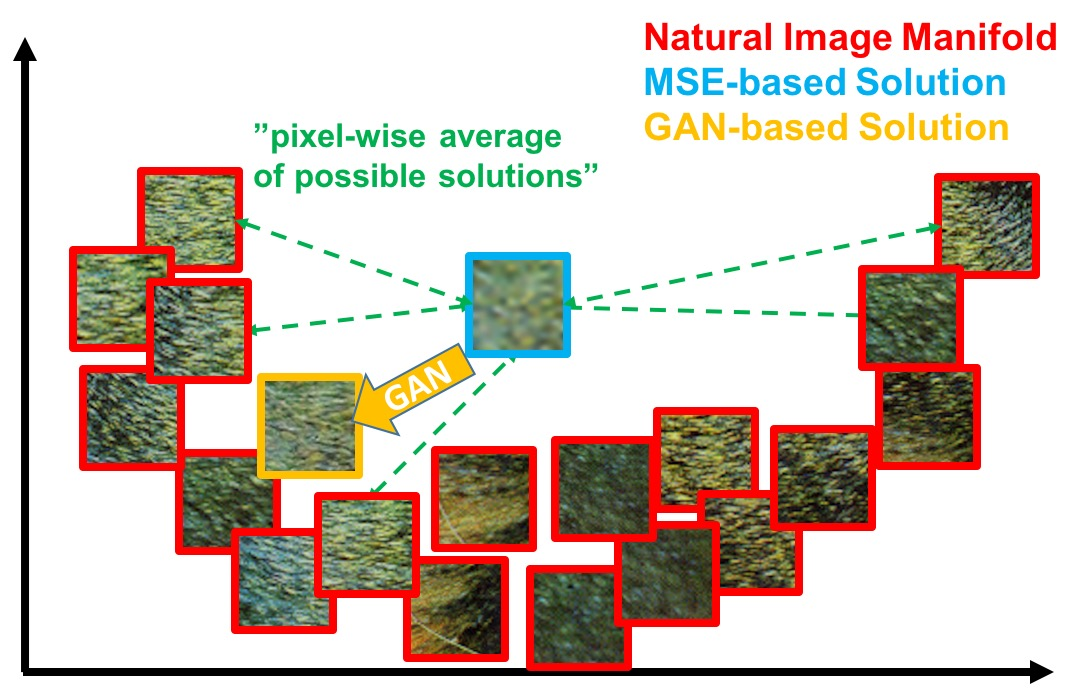
\includegraphics[trim=0 0 0 0, clip, width=3.1in]{images/used/jpg/manifold.jpg}
\caption{\eng{
Illustration of patches from the natural image manifold (red) and super-resolved patches obtained with MSE (blue) and GAN (orange).
}\kor{
자연 이미지 데이터 공간(manifold)에서 얻어진 패치 (적색), MSE로 초해상도화하여 얻어진 패치 (청색), GAN을 이용해서 얻은 패치 (주황색)들의 사진
} \eng{
The MSE-based solution appears overly smooth due to the pixel-wise average of possible solutions in the pixel space, while GAN drives the reconstruction towards the natural image manifold producing perceptually more convincing solutions.
}\kor{
MSE 기반 방법은 픽셀 공간에서 가능한 해의 픽셀 단위(pixel-wise) 평균으로 인해 과하게 매끄럽게 보이는 반면, GAN은 자연 이미지 데이터 공간(manifold)쪽으로 재구성을 유도해서, 지각적으로 더욱 실감나는 해를 생성한다.
}}
\label{fig:manifold}
\end{figure}

\subsubsection{\eng{Loss functions}\kor{손실 함수}}
\eng{
Pixel-wise loss functions such as \ac{MSE} struggle to handle the uncertainty inherent in recovering lost high-frequency details such as texture: minimizing \ac{MSE} encourages finding pixel-wise averages of plausible solutions which are typically overly-smooth and thus have poor perceptual quality \cite{Mathieu2015, Johnson16PercepLoss, dosovitskiy2016generating, bruna2016super}.
}\kor{
\ac{MSE}와 같은 픽셀 단위 손실 함수는 질감과 같은 손실된 고주파 세부 정보를 복구할 때, 내재된 불확실성을 처리하기 위해 노력한다: \ac{MSE}를 최소화하는 것은 일반적으로 지나치게 매끄러워서, 나쁜 지각적 품질을 가지는 그럴듯한 해를 찾는 것을 촉진한다\cite{Mathieu2015, Johnson16PercepLoss, dosovitskiy2016generating, bruna2016super}.
}
\eng{
Reconstructions of varying perceptual quality are exemplified with corresponding \ac{PSNR} in \figurename~\ref{fig:exampleIntro}.
}\kor{
다양한 지각 품질의 재구성 결과는 \figurename~\ref{fig:exampleIntro}에서 \ac{PSNR}과 함께 확인할 수 있다.
} \eng{
We illustrate the problem of minimizing \ac{MSE} in \figurename~\ref{fig:manifold} where multiple potential solutions with high texture details are averaged to create a smooth reconstruction.
}\kor{
높은 질감 세부 사항의 여러 잠재적 해가 평균화되어 매끄러운 복원물을 만드는 \figurename~\ref{fig:manifold}에서는 \ac{MSE}를 최소화하는 문제를 설명한다.
}

\eng{
In Mathieu et al. \cite{Mathieu2015} and Denton et al. \cite{Denton2015} the authors tackled this problem by employing \acp{GAN} \cite{Goodfellow14GAN} for the application of image generation.
}\kor{
Mathieu 외. \cite{Mathieu2015}와 Denton 외. \cite{Denton2015}에서 저자들은 이미지 생성의 응용을 위해 \acp{GAN} \cite{Goodfellow14GAN}을 사용함으로써 이 문제를 해결했다.
} \eng{
Yu and Porikli \cite{yu2016ultra} augment pixel-wise \ac{MSE} loss with a discriminator loss to train a network that super-resolves face images with large upscaling factors ($8\times$).
}\kor{
Yu와 Porikli \cite{yu2016ultra}는 큰 해상도 향상 인자($8\times$)로 얼굴 이미지를 초해상도화하는 네트워크를 훈련시키기 위해 판별기(discriminator) 손실과 함께 픽셀 단위의 \ac{MSE} 손실을 증가시켰다.
} \eng{
\acp{GAN} were also used for unsupervised representation learning in Radford et al. \cite{Radford2015}.
}\kor{
\acp{GAN}은 Radford 외. \cite{Radford2015}의 비지도 표현 학습에도 사용되었다.
}
\eng{
The idea of using \acp{GAN} to learn a mapping from one manifold to another is described by Li and Wand \cite{Li2016} for style transfer and Yeh et al. \cite{Yeh2016} for inpainting.
}\kor{
한 데이터 공간(manifold)에서 다른 데이터 공간(manifold)로의 사상(mapping)을 학습하기 위해 GAN을 사용하는 아이디어는 스타일 전이를 위한 Li와 Wand \cite{Li2016}와 이미지 복원(inpainting)을 위한 Yeh 외. \cite{Yeh2016}에서 설명된다.
}
\eng{
Bruna et al. \cite{bruna2016super} minimize the squared error in the feature spaces of VGG19 \cite{simonyan2014very} and scattering networks.
}\kor{
Bruna 외. \cite{bruna2016super}는 VGG19의 특징 공간과 산란 네트워크에서 제곱 오차를 최소화한다.
}

Dosovitskiy and Brox \cite{dosovitskiy2016generating} use loss functions based on Euclidean distances computed in the feature space of neural networks in combination with adversarial training. It is shown that the proposed loss allows visually superior image generation and can be used to solve the ill-posed inverse problem of decoding nonlinear feature representations.
Similar to this work, Johnson et al. \cite{Johnson16PercepLoss} and Bruna et al. \cite{bruna2016super} propose the use of features extracted from a pre-trained VGG network instead of low-level pixel-wise error measures. Specifically the authors formulate a loss function based on the euclidean distance between feature maps extracted from the VGG19 \cite{simonyan2014very} network. Perceptually more convincing results were obtained for both super-resolution and artistic style-transfer \cite{Gatys2015nips,Gatys2016cvpr}. Recently, Li and Wand \cite{Li2016} also investigated the effect of comparing and blending patches in pixel or VGG feature space.

\subsection{Contribution}
\acp{GAN} provide a powerful framework for generating plausible-looking natural images with high perceptual quality.
%In the \ac{GAN} framework, two neural networks, a generator and a discriminator, are trained simultaneously with competing goals. The discriminator network is trained to distinguish natural and synthetically generated images, while the generator learns to generate images that are indistinguishable from natural images by the best discriminator.
The \ac{GAN} procedure encourages the reconstructions to move towards regions of the search space with high probability of containing photo-realistic images and thus closer to the natural image manifold as shown in \figurename~\ref{fig:manifold}.

In this paper we describe the first very deep \ac{ResNet} \cite{he2015deep,he2016identity} architecture using the concept of \acp{GAN} to form a perceptual loss function for photo-realistic \ac{SISR}. Our main contributions are:
\begin{itemize}
\item We set a new state of the art for image \ac{SR} with high upscaling factors ($4\times$) as measured by \ac{PSNR} and \ac{SSIM} with our 16 blocks deep \ac{ResNet} (SRResNet) optimized for \ac{MSE}. %Specifically, we employ the fast feature learning in \ac{LR} space \cite{Shi2016ESPCN,Johnson16PercepLoss} and batch-normalization \cite{Ioffe2015} to robustly train a network of 16 residual blocks for better accuracy.
\item We propose SRGAN which is a \ac{GAN}-based network optimized for a new perceptual loss. Here we replace the \ac{MSE}-based content loss with a loss calculated on feature maps of the VGG network \cite{simonyan2014very}, which are more invariant to changes in pixel space \cite{Li2016}. %as illustrated in Figures 3 and 4 in Li and Wand .
\item We confirm with an extensive \ac{MOS} test on images from three public benchmark datasets that SRGAN is the new state of the art, by a large margin, for the estimation of photo-realistic \ac{SR} images with high upscaling factors ($4\times$).
\end{itemize}

%The adversarial loss is driven by a discriminator network to encourage solutions from the natural image domain while the content loss ensures that the super-resolved images have the same content as their low-resolution counterparts. We further replace the \ac{MSE}-based content loss function with the euclidean distance between the last convolutional feature maps of the VGG network \cite{simonyan2014very}, which are more invariant to changes in pixel space as illustrated in Figures 3 and 4 in Li and Wand \cite{Li2016}.
% We validate the proposed approaches using images from three publicly available benchmark.
%datasets and compare the performance against state-of-the-art works.
%including SRCNN \cite{dong2014learning}, SelfExSR \cite{Huang15selfexemplars} and \ac{DRCN} \cite{kim2016deeply}. We confirm our network's potential to reconstruct photo-realistic images under $4\times$ downsampling factors using standard measures and extensive MOS testing.

We describe the network architecture and the perceptual loss in Section \ref{sec:method}. A quantitative evaluation on public benchmark datasets as well as visual illustrations are provided in Section \ref{sec:experiments}. The paper concludes with a discussion in Section \ref{sec:discussion} and concluding remarks in Section \ref{sec:conclusion}.

\section{Method}
\label{sec:method}

\begin{figure*}[ht!]
\begin{center}
\begin{tabular}{c}
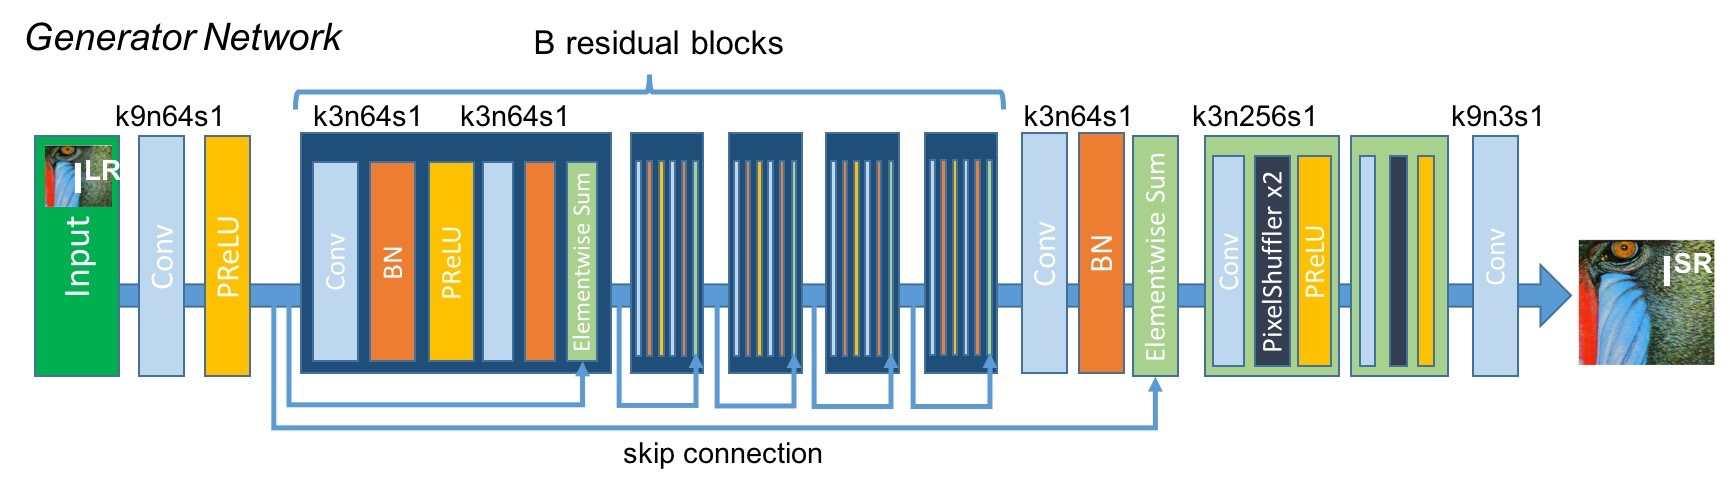
\includegraphics[width=6.5in]{images/used/jpg/generator}\\
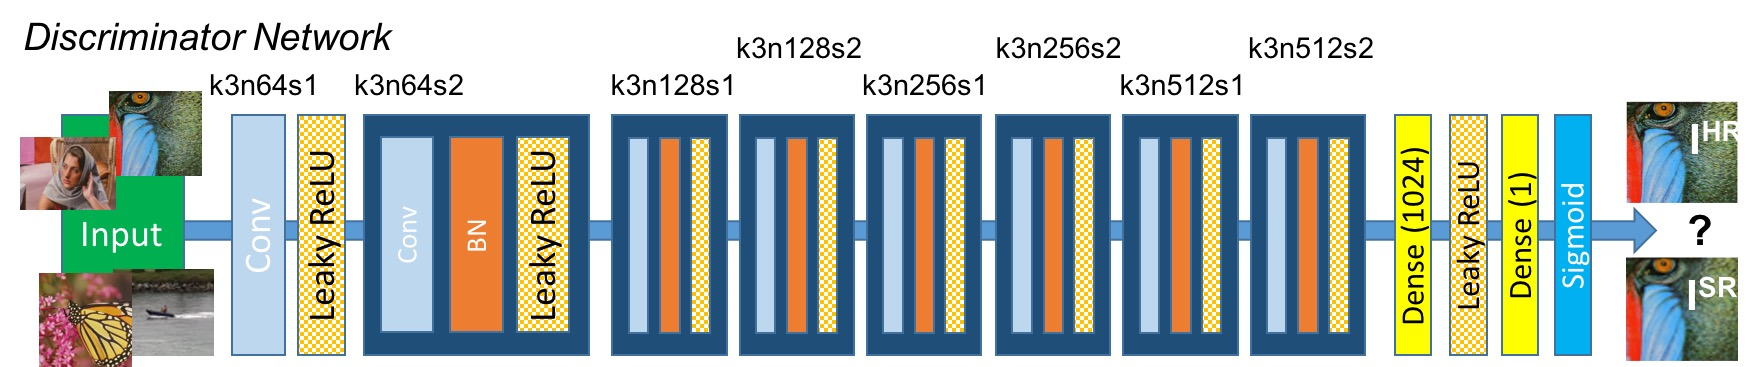
\includegraphics[width=6.5in]{images/used/jpg/discriminator}
\end{tabular}
\end{center}
\caption{Architecture of Generator and Discriminator Network with corresponding kernel size (k), number of feature maps (n) and stride (s) indicated for each convolutional layer.}
\label{fig:generator}
\end{figure*}
%
In \ac{SISR} the aim is to estimate a high-resolution, super-resolved image $I^{SR}$ from a low-resolution input image $I^{LR}$. Here $I^{LR}$ is the low-resolution version of its high-resolution counterpart $I^{HR}$. The high-resolution images are only available during training. In training, $I^{LR}$ is obtained by applying a Gaussian filter to $I^{HR}$ followed by a downsampling operation with downsampling factor $r$. For an image with $C$ color channels, we describe $I^{LR}$ by a real-valued tensor of size $W \times H \times C$ and $I^{HR}$, $I^{SR}$ by $rW \times rH \times C$ respectively.

Our ultimate goal is to train a generating function $G$ that estimates for a given \ac{LR} input image its corresponding \ac{HR} counterpart. To achieve this, we train a generator network as a feed-forward \ac{CNN} $G_{\theta_G}$ parametrized by ${\theta_G}$. Here ${\theta_G}=\{W_{1:L}; b_{1:L}\}$ denotes the weights and biases of a $L$-layer deep network and is obtained by optimizing a SR-specific loss function $l^{SR}$. For training images $I^{HR}_n$ , $n = 1,\dots,N$ with corresponding $I^{LR}_n$ , $n = 1,\dots,N$, we solve:
\begin{equation}
\hat{{\theta}}_G = \arg\min_{\theta_G} \frac{1}{N} \sum_{n=1}^{N}{l^{SR}(G_{\theta_G}(I^{LR}_n),I^{HR}_n)}
\end{equation}
In this work we will specifically design a perceptual loss $l^{SR}$ as a weighted combination of several loss components that model distinct desirable characteristics of the recovered \ac{SR} image. The individual loss functions are described in more detail in Section \ref{sec:losses}.

\subsection{Adversarial network architecture}
Following Goodfellow et al. \cite{Goodfellow14GAN} we further define a discriminator network $D_{\theta_D}$ which we optimize in an alternating manner along with $G_{\theta_G}$ to solve the adversarial min-max problem:
\begin{equation}
\label{eq:minmax}
\begin{split}
\min_{\theta_G} \max_{\theta_D} ~& \mathbb{E}_{I^{HR}\sim p_\textrm{train}(I^{HR})} [ \log D_{\theta_D}(I^{HR}) ] + \\
& \mathbb{E}_{I^{LR}\sim p_G(I^{LR})} [ \log (1-D_{\theta_D}(G_{\theta_G}(I^{LR})) ]
\end{split}
\end{equation}
The general idea behind this formulation is that it allows one to train a generative model $G$ with the goal of fooling a differentiable discriminator $D$ that is trained to distinguish super-resolved images from real images.
With this approach our generator can learn to create solutions that are highly similar to real images and thus difficult to classify by $D$. This encourages perceptually superior solutions residing in the subspace, the manifold, of natural images. This is in contrast to \ac{SR} solutions obtained by minimizing pixel-wise error measurements, such as the \ac{MSE}.

At the core of our very deep generator network $G$, which is illustrated in \figurename~\ref{fig:generator} are $B$ residual blocks with identical layout. Inspired by Johnson et al. \cite{Johnson16PercepLoss} we employ the block layout proposed by Gross and Wilber \cite{gross2016}. Specifically, we use two convolutional layers with small $3\times3$ kernels and 64 feature maps followed by batch-normalization layers \cite{Ioffe2015} and ParametricReLU \cite{He2015relu} as the activation function.
We increase the resolution of the input image with two trained sub-pixel convolution layers as proposed by Shi et al. \cite{Shi2016ESPCN}.

To discriminate real \ac{HR} images from generated \ac{SR} samples we train a discriminator network. The architecture is shown in \figurename~\ref{fig:generator}.
We follow the architectural guidelines summarized by Radford et al. \cite{Radford2015} and use LeakyReLU activation ($\alpha=0.2$) and avoid max-pooling throughout the network. The discriminator network is trained to solve the maximization problem in Equation \ref{eq:minmax}. It contains eight convolutional layers with an increasing number of $3\times3$ filter kernels, increasing by a factor of 2 from 64 to 512 kernels as in the VGG network \cite{simonyan2014very}. Strided convolutions are used to reduce the image resolution each time the number of features is doubled. The resulting 512 feature maps are followed by two dense layers and a final sigmoid activation function to obtain a probability for sample classification.

\subsection{Perceptual loss function}
\label{sec:losses}
The definition of our perceptual loss function $l^{SR}$  is critical for the performance of our generator network.
While $l^{SR}$ is commonly modeled based on the \ac{MSE}  \cite{dong2016image,Shi2016ESPCN}, we improve on Johnson et al. \cite{Johnson16PercepLoss} and Bruna et al. \cite{bruna2016super} and design a loss function that assesses a solution with respect to perceptually relevant characteristics.
We formulate the perceptual loss as the weighted sum of a content loss ($l^{SR}_\textrm{X}$) and an adversarial loss component as:

\begin{equation}
l^{SR} = \underbrace{\underbrace{l^{SR}_\textrm{X}}_{\text{content loss}} + \underbrace{10^{-3} l^{SR}_{Gen}}_{\text{adversarial loss}}}_{\text{perceptual loss (for VGG based content losses)}}
\end{equation}
In the following we describe possible choices for the content loss $l^{SR}_\textrm{X}$ and the adversarial loss $l^{SR}_\textrm{Gen}$.

\subsubsection{Content loss}

The pixel-wise \textbf{\ac{MSE} loss} is calculated as:
\begin{equation}
l^{SR}_{MSE} = \frac{1}{r^2WH} \sum_{x=1}^{rW} \sum_{y=1}^{rH} (I^{HR}_{x,y} - G_{\theta_G}(I^{LR})_{x,y})^2
\end{equation}
This is the most widely used optimization target for image \ac{SR} on which many state-of-the-art approaches rely \cite{dong2016image,Shi2016ESPCN}. However, while achieving particularly high \ac{PSNR}, solutions of \ac{MSE} optimization problems often lack high-frequency content which results in perceptually unsatisfying solutions with overly smooth textures (\cf \figurename~\ref{fig:exampleIntro}).

Instead of relying on pixel-wise losses we build on the ideas of Gatys et al. \cite{Gatys2015nips}, Bruna et al. \cite{bruna2016super} and Johnson et al. \cite{Johnson16PercepLoss} and use a loss function that is closer to perceptual similarity. We define the \textbf{VGG loss} based on the ReLU activation layers of the pre-trained 19 layer VGG network described in Simonyan and Zisserman \cite{simonyan2014very}. With $\phi_{i,j}$ we indicate the feature map obtained by the j-th convolution (after activation) before the i-th maxpooling layer within the VGG19 network, which we consider given.
We then define the VGG loss as the euclidean distance between the feature representations of a reconstructed image $G_{\theta_G}(I^{LR})$ and the reference image $I^{HR}$:
\begin{equation}
\begin{split}
l^{SR}_{VGG/i.j} =
\frac{1}{W_{i,j}H_{i,j}} & \sum_{x=1}^{W_{i,j}} \sum_{y=1}^{H_{i,j}} (\phi_{i,j}(I^{HR})_{x,y} \\
& - \phi_{i,j}(G_{\theta_G}(I^{LR}))_{x,y})^2
\end{split}
\label{eq:vgg}
\end{equation}

Here $W_{i,j}$ and $H_{i,j}$ describe the dimensions of the respective feature maps within the VGG network.

\subsubsection{Adversarial loss}
In addition to the content losses described so far, we also add the generative component of our \ac{GAN} to the perceptual loss. This encourages our network to favor solutions that reside on the manifold of natural images, by trying to fool the discriminator network. The generative loss $l^{SR}_{Gen}$ is defined based on the probabilities of the discriminator $D_{\theta_D}(G_{\theta_G}(I^{LR}))$ over all training samples as:
\begin{equation}
l^{SR}_{Gen} = \sum_{n=1}^{N} -\log D_{\theta_D}(G_{\theta_G}(I^{LR}))
\end{equation}

Here, $D_{\theta_D}(G_{\theta_G}(I^{LR}))$ is the probability that the
reconstructed image $G_{\theta_G}(I^{LR})$ is a natural HR image. For better gradient behavior we minimize $-\log D_{\theta_D}(G_{\theta_G}(I^{LR}))$ instead of $\log [1-D_{\theta_D}(G_{\theta_G}(I^{LR}))]$ \cite{Goodfellow14GAN}.

%
\section{Experiments}
\label{sec:experiments}
\subsection{Data and similarity measures}
\label{subsec:data}
We perform experiments on three widely used benchmark datasets \textbf{Set5} \cite{bevilacqua2012low}, \textbf{Set14} \cite{zeyde2012single} and \textbf{BSD100}, the testing set of BSD300 \cite{MartinFTM01}. All experiments are performed with a scale factor of $4\times$ between low- and high-resolution images. This corresponds to a $16\times$ reduction in image pixels. For fair comparison, all reported \ac{PSNR} [dB] and \ac{SSIM} \cite{Wang2004} measures were calculated on the y-channel of center-cropped, removal of a 4-pixel wide strip from each border, images using the daala package\footnote{\url{https://github.com/xiph/daala} (commit: 8d03668)}. Super-resolved images for the reference methods, including nearest neighbor, bicubic, SRCNN \cite{dong2014learning} and SelfExSR \cite{Huang15selfexemplars}, were obtained from online material supplementary to Huang et al.\footnote{\url{https://github.com/jbhuang0604/SelfExSR}} \cite{Huang15selfexemplars} and for DRCN from Kim et al.\footnote{\url{http://cv.snu.ac.kr/research/DRCN/}} \cite{kim2016deeply}.
Results obtained with SRResNet (for losses: $l^{SR}_{MSE}$ and $l^{SR}_{VGG/2.2}$) and the SRGAN variants are available online\footnote{\url{https://twitter.box.com/s/lcue6vlrd01ljkdtdkhmfvk7vtjhetog}}.
Statistical tests were performed as paired two-sided Wilcoxon signed-rank tests and significance determined at $p<0.05$.

The reader may also be interested in an independently developed GAN-based solution on GitHub\footnote{\url{https://github.com/david-gpu/srez}}. However it only provides experimental results on a limited set of faces, which is a more constrained and easier task.

\subsection{Training details and parameters}
We trained all networks on a NVIDIA Tesla M40 GPU using a random sample of 350 thousand images from the \textbf{ImageNet} database \cite{russakovsky2014imagenet}. These images are distinct from the testing images. We obtained the \ac{LR} images by downsampling the \ac{HR} images (BGR, $C=3$) using bicubic kernel with downsampling factor $r=4$. For each mini-batch we crop 16 random $96\times96$ \ac{HR} sub images of distinct training images. Note that we can apply the generator model to images of arbitrary size as it is fully convolutional.
We scaled the range of the \ac{LR} input images to $[0, 1]$ and for the \ac{HR} images to $[-1, 1]$. The \ac{MSE} loss was thus calculated on images of intensity range $[-1, 1]$. VGG feature maps were also rescaled by a factor of $\frac{1}{12.75}$ to obtain VGG losses of a scale that is comparable to the \ac{MSE} loss. This is equivalent to multiplying Equation \ref{eq:vgg} with a rescaling factor of $\approx0.006$.
For optimization we use Adam \cite{Kingma2014} with $\beta_1=0.9$. The SRResNet networks were trained with a learning rate of $10^{-4}$ and $10^{6}$ update iterations. We employed the trained \ac{MSE}-based SRResNet network as initialization for the generator when training the actual \ac{GAN} to avoid undesired local optima.
All SRGAN variants were trained with $10^5$ update iterations at a learning rate of $10^{-4}$ and another $10^5$ iterations at a lower rate of $10^{-5}$.
We alternate updates to the generator and discriminator network, which is equivalent to $k=1$ as used in Goodfellow et al. \cite{Goodfellow14GAN}. Our generator network has 16 identical ($B=16$) residual blocks. During test time we turn batch-normalization update off to obtain an output that deterministically depends only on the input \cite{Ioffe2015}. Our implementation is based on Theano \cite{theano2016} and Lasagne \cite{lasagne2015}.

\subsection{Mean opinion score (MOS) testing}
We have performed a \ac{MOS} test to quantify the ability of different approaches to reconstruct perceptually convincing images. Specifically, we asked 26 raters to assign an integral score from 1 (bad quality) to 5 (excellent quality) to the super-resolved images. The raters rated 12 versions of each image on \textbf{Set5}, \textbf{Set14} and \textbf{BSD100}: nearest neighbor (NN), bicubic, SRCNN \cite{dong2014learning}, SelfExSR \cite{Huang15selfexemplars}, DRCN \cite{kim2016deeply}, ESPCN \cite{Shi2016ESPCN}, \textbf{SRResNet}-MSE, SRResNet-VGG22$^\ast$ ($^\ast$not rated on \textbf{BSD100}), SRGAN-MSE$^\ast$, SRGAN-VGG22$^\ast$, \textbf{SRGAN}-VGG54 and the original HR image. Each rater thus rated 1128 instances (12 versions of 19 images plus 9 versions of 100 images) that were presented in a randomized fashion.
The raters were calibrated on the NN (score 1) and HR (5) versions of 20 images from the BSD300 training set.
In a pilot study we assessed the calibration procedure and the test-retest reliability of 26 raters on a subset of 10 images from BSD100 by adding a method's images twice to a larger test set. We found good reliability and no significant differences between the ratings of the identical images.
Raters very consistently rated NN interpolated test images as 1 and the original HR images as 5 (\cf \figurename~\ref{fig:MOS}).

The experimental results of the conducted \ac{MOS} tests are summarized in Table \ref{tab:perceptual}, Table \ref{tab:performance} and \figurename~\ref{fig:MOS}.

\begin{table}[]
\centering
\caption{Performance of different loss functions for SRResNet and the adversarial networks on Set5 and Set14 benchmark data. MOS score significantly higher ($p<0.05$) than with other losses in that category$^*$. [$4\times$ upscaling]}
\label{tab:perceptual}
\begin{adjustbox}{max width=0.48\textwidth}
\begin{tabular}{lll | lll}
& \multicolumn{2}{c}{SRResNet-} & \multicolumn{3}{c}{SRGAN-} \\
\textbf{Set5} & MSE & VGG22 & MSE & VGG22 & VGG54 \\
\hline

PSNR &  32.05 & 30.51 & 30.64 & 29.84 & 29.40 \\
SSIM & 0.9019 & 0.8803 & 0.8701 & 0.8468 & 0.8472 \\
MOS  &  3.37 & 3.46 & 3.77 & 3.78 & 3.58 \\ [0.3cm]
\textbf{Set14} & & &  \\
\hline
PSNR &  28.49 & 27.19 & 26.92 & 26.44 & 26.02 \\
SSIM &  0.8184 & 0.7807 & 0.7611 & 0.7518 & 0.7397 \\
MOS  &  2.98 & 3.15$^*$ & 3.43 & 3.57 & 3.72$^*$  \\
%\textbf{BSD100} & & &  \\
%\hline
%PSNR &  25.95 & 25.67 & 25.16 \\
%SSIM &  0.6698 & 0.6852 & 0.6688 \\
\end{tabular}
\end{adjustbox}
\end{table}
\subsection{Investigation of content loss}
We investigated the effect of different content loss choices in the perceptual loss for the \ac{GAN}-based networks. Specifically we investigate $l^{SR} = l^{SR}_\textrm{X} + 10^{-3}l^{SR}_{Gen}$ for the following content losses $l^{SR}_\textrm{X}$:\\
\begin{itemize}
\item SRGAN-MSE: $l^{SR}_{MSE}$, to investigate the adversarial network with the standard \ac{MSE} as content loss.
\item SRGAN-VGG22: $l^{SR}_{VGG/2.2}$ with $\phi_{2,2}$, a loss defined on feature maps representing lower-level features \cite{zeiler2014visualizing}.
\item \textbf{SRGAN}-VGG54: $l^{SR}_{VGG/5.4}$ with $\phi_{5,4}$, a loss defined on feature maps of higher level features from deeper network layers with more potential to focus on the content of the images \cite{zeiler2014visualizing,Yosinski2015,Mahendran2016}. We refer to this network as \textbf{SRGAN} in the following.
\end{itemize}
We also evaluate the performance of the generator network without adversarial component for the two losses $l^{SR}_{MSE}$ (\textbf{SRResNet}-MSE) and $l^{SR}_{VGG/2.2}$ (SRResNet-VGG22). We refer to SRResNet-MSE as \textbf{SRResNet}.
Note, when training SRResNet-VGG22 we added an additional total variation loss with weight $2\times10^{-8}$ to $l^{SR}_{VGG/2.2}$ \cite{Aly2005,Johnson16PercepLoss}.
Quantitative results are summarized in Table \ref{tab:perceptual} and visual examples provided in \figurename~\ref{fig:perceptual}.
Even combined with the adversarial loss, \ac{MSE} provides solutions with the highest \ac{PSNR} values that are, however, perceptually rather smooth and less convincing than results achieved with a loss component more sensitive to visual perception. This is caused by competition between the \ac{MSE}-based content loss and the adversarial loss. We further attribute minor reconstruction artifacts, which we observed in a minority of SRGAN-MSE-based reconstructions, to those competing objectives. We could not determine a significantly best loss function for SRResNet or SRGAN with respect to \ac{MOS} score on \textbf{Set5}. However, \textbf{SRGAN}-VGG54 significantly outperformed other SRGAN and SRResNet variants on \textbf{Set14} in terms of \ac{MOS}.
We observed a trend that using the higher level VGG feature maps $\phi_{5,4}$ yields better texture detail when compared to $\phi_{2,2}$ (\cf \figurename~\ref{fig:perceptual}).
Further examples of perceptual improvements through \textbf{SRGAN} over \textbf{SRResNet} are provided in the supplementary material.
\begin{figure}[ht!]
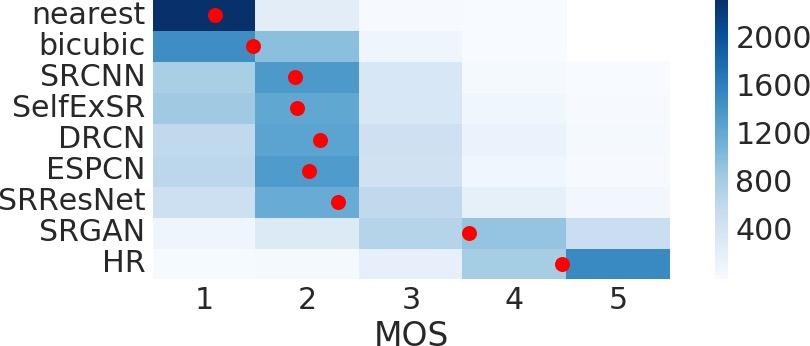
\includegraphics[width=0.48\textwidth]{images/used/jpg/MOS_heatmapcropped}
\caption{Color-coded distribution of MOS scores on \textbf{BSD100}. For each method 2600 samples (100 images $\times$ 26 raters) were assessed. Mean shown as red marker, where the bins are centered around value $i$. [$4\times$ upscaling]}
\label{fig:MOS}
\end{figure}

\begin{figure*}[ht!]
\begin{tabular}{ cx{3.7cm}cx{3.7cm}cx{3.7cm}cx{3.7cm}cx{3.7cm}}
~~~~~~~~~\textbf{SRResNet} & ~~~~~~~SRGAN-MSE & ~SRGAN-VGG22 & \textbf{SRGAN}-VGG54 & original HR image \\
\end{tabular}

\begin{tikzpicture}[zoomboxarray, zoomboxes below, zoomboxarray inner gap=0.1cm, zoomboxarray columns=2, zoomboxarray rows=2]
\node [image node] { 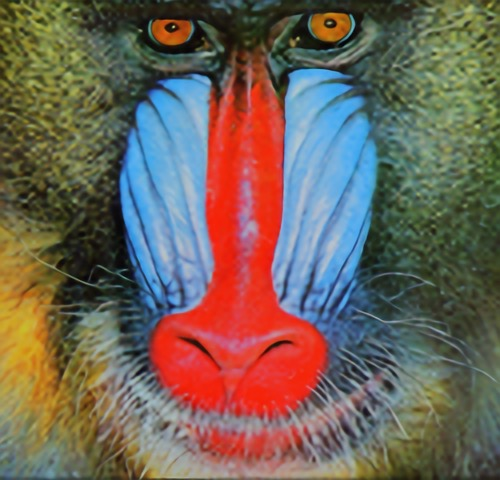
\includegraphics[trim=200 220 40 5, clip, width=1.3in]{images/used/jpg/baboon_SRResNet-MSE} };
\zoombox[magnification=2,color code=red]{0.5,0.85}
\zoombox[magnification=2,color code=yellow]{0.7,0.55}
\zoombox[magnification=2,color code=orange]{0.35,0.3}
\zoombox[magnification=5,color code=lime]{0.86,0.25}
\end{tikzpicture}
\begin{tikzpicture}[zoomboxarray, zoomboxes below, zoomboxarray inner gap=0.1cm, zoomboxarray columns=2, zoomboxarray rows=2]
\node [image node] { 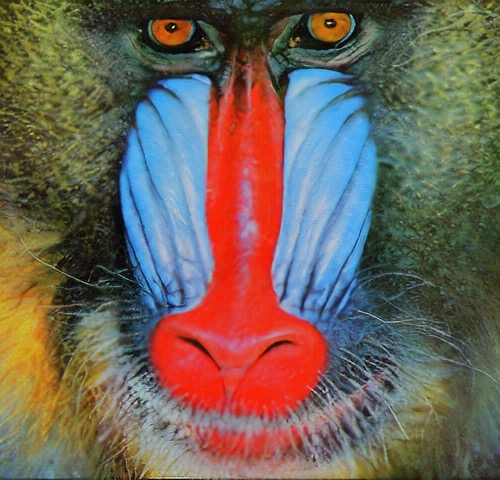
\includegraphics[trim=200 220 40 5, clip, width=1.3in]{images/used/jpg/baboon_SRGAN-MSE} };
\zoombox[magnification=2,color code=red]{0.5,0.85}
\zoombox[magnification=2,color code=yellow]{0.7,0.55}
\zoombox[magnification=2,color code=orange]{0.35,0.3}
\zoombox[magnification=5,color code=lime]{0.86,0.25}
\end{tikzpicture}
\begin{tikzpicture}[zoomboxarray, zoomboxes below, zoomboxarray inner gap=0.1cm, zoomboxarray columns=2, zoomboxarray rows=2]
\node [image node] { 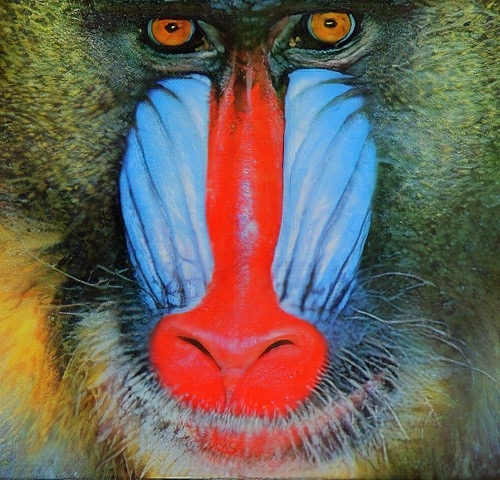
\includegraphics[trim=200 220 40 5, clip, width=1.3in]{images/used/jpg/baboon_SRGAN-VGG22} };
\zoombox[magnification=2,color code=red]{0.5,0.85}
\zoombox[magnification=2,color code=yellow]{0.7,0.55}
\zoombox[magnification=2,color code=orange]{0.35,0.3}
\zoombox[magnification=5,color code=lime]{0.86,0.25}
\end{tikzpicture}
\begin{tikzpicture}[zoomboxarray, zoomboxes below, zoomboxarray inner gap=0.1cm, zoomboxarray columns=2, zoomboxarray rows=2]
\node [image node] { 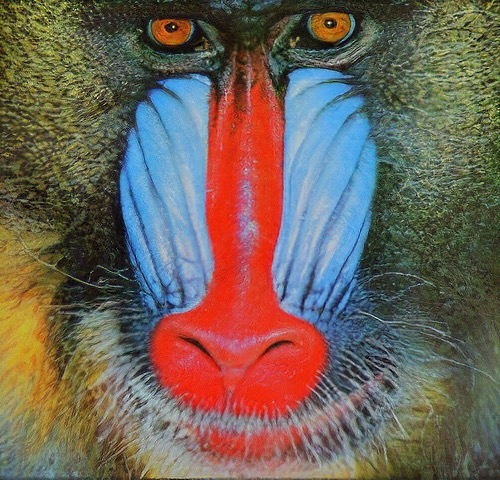
\includegraphics[trim=200 220 40 5, clip, width=1.3in]{images/used/jpg/baboon_SRGAN-VGG54} };
\zoombox[magnification=2,color code=red]{0.5,0.85}
\zoombox[magnification=2,color code=yellow]{0.7,0.55}
\zoombox[magnification=2,color code=orange]{0.35,0.3}
\zoombox[magnification=5,color code=lime]{0.86,0.25}
\end{tikzpicture}
\begin{tikzpicture}[zoomboxarray, zoomboxes below, zoomboxarray inner gap=0.1cm, zoomboxarray columns=2, zoomboxarray rows=2]
\node [image node] { 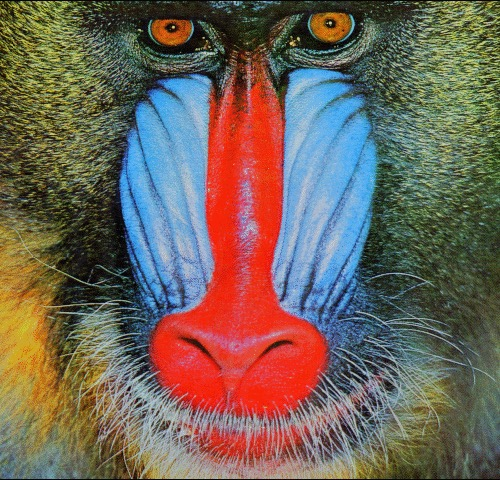
\includegraphics[trim=200 220 40 5, clip, width=1.3in]{images/used/jpg/baboon_HR} };
\zoombox[magnification=2,color code=red]{0.5,0.85}
\zoombox[magnification=2,color code=yellow]{0.7,0.55}
\zoombox[magnification=2,color code=orange]{0.35,0.3}
\zoombox[magnification=5,color code=lime]{0.86,0.25}
\end{tikzpicture}
\caption{\textbf{SRResNet} (left: a,b), SRGAN-MSE (middle left: c,d), SRGAN-VGG2.2 (middle: e,f) and  \textbf{SRGAN}-VGG54 (middle right: g,h) reconstruction results and corresponding reference HR image (right: i,j). [$4\times$ upscaling]}
\label{fig:perceptual}
\end{figure*}

\begin{table*}[htb!]
\centering
\caption{Comparison of NN, bicubic, SRCNN \cite{dong2014learning}, SelfExSR \cite{Huang15selfexemplars}, DRCN \cite{kim2016deeply}, ESPCN \cite{Shi2016ESPCN}, \textbf{SRResNet}, \textbf{SRGAN}-VGG54 and the original HR on benchmark data. Highest measures (PSNR [dB], SSIM, MOS) in bold. [$4\times$ upscaling]}
\label{tab:performance}
\begin{adjustbox}{max width=0.8\textwidth}
\begin{tabular}{llllllllll}
\textbf{Set5} & nearest & bicubic & SRCNN & SelfExSR & DRCN & ESPCN & \textbf{SRResNet} & \textbf{SRGAN} & HR \\
\hline
PSNR & 26.26 & 28.43 & 30.07 & 30.33 & 31.52 & 30.76 & \textbf{32.05} & 29.40 & $\infty$ \\
SSIM & 0.7552 & 0.8211 & 0.8627 & 0.872 & 0.8938 & 0.8784 & \textbf{0.9019} & 0.8472 & 1 \\
MOS  & 1.28 & 1.97 & 2.57 & 2.65 & 3.26 & 2.89 & 3.37 & \textbf{3.58} & 4.32 \\ [0.3cm]

\textbf{Set14} & & & & & & & & \\
\hline
PSNR & 24.64 & 25.99 & 27.18 & 27.45 & 28.02 & 27.66 & \textbf{28.49} & 26.02 & $\infty$ \\
SSIM & 0.7100 & 0.7486 & 0.7861 & 0.7972 & 0.8074 & 0.8004 & \textbf{0.8184} & 0.7397 & 1 \\
MOS  & 1.20 & 1.80 & 2.26 & 2.34 & 2.84 & 2.52 & 2.98 & \textbf{3.72} & 4.32 \\ [0.3cm]
\textbf{BSD100} & & & & & & & &  \\
\hline
PSNR & 25.02 & 25.94 & 26.68 & 26.83 & 27.21 & 27.02 & \textbf{27.58} & 25.16 & $\infty$ \\
SSIM & 0.6606 & 0.6935 & 0.7291 & 0.7387 & 0.7493 & 0.7442 & \textbf{0.7620} & 0.6688 & 1 \\
MOS  & 1.11 & 1.47 & 1.87 & 1.89 & 2.12 & 2.01 & 2.29 & \textbf{3.56} & 4.46 \\
\end{tabular}
\end{adjustbox}
\end{table*}

\subsection{Performance of the final networks}
\label{subsec:msebased}
%In this paper, we choose a network architecture for the generator (cf. Figure \ref{fig:generator}) which combines the effectiveness of the \ac{ESPCN} \cite{Shi2016ESPCN} and the high performance of the \ac{ResNet} \cite{he2015deep}.
We compare the performance of \textbf{SRResNet} and \textbf{SRGAN} to NN, bicubic interpolation, and four state-of-the-art methods.
%: the super-resolution \ac{CNN} (SRCNN) described by Dong et al. \cite{dong2014learning}, a method based on transformed self-exemplars (SelfExSR) \cite{Huang15selfexemplars}, a deeply-recursive convolutional network (DRCN) described by Kim et al. \cite{kim2016deeply} and the efficient sub-pixel \ac{CNN} (ESPCNN) allowing real-time video \ac{SR} \cite{Shi2016ESPCN}.
Quantitative results are summarized in Table \ref{tab:performance} and confirm that \textbf{SRResNet} (in terms of PSNR/SSIM) sets a new state of the art on three benchmark datasets.
Please note that we used a publicly available framework for evaluation (\cf Section \ref{subsec:data}), reported values might thus slightly deviate from those reported in the original papers.

We further obtained \ac{MOS} ratings for \textbf{SRGAN} and all reference methods on \textbf{BSD100}. Examples of images super-resolved with \textbf{SRResNet} and \textbf{SRGAN} are depicted in the supplementary material.
The results shown in Table \ref{tab:performance} confirm that \textbf{SRGAN} outperforms all reference methods by a large margin and sets a new state of the art for photo-realistic image \ac{SR}. All differences in \ac{MOS} (\cf Table \ref{tab:performance}) are highly significant on \textbf{BSD100}, except SRCNN vs. SelfExSR. The distribution of all collected \ac{MOS} ratings is summarized in \figurename~\ref{fig:MOS}.

\section{Discussion and future work}
\label{sec:discussion}
We confirmed the superior perceptual performance of \textbf{SRGAN} using \ac{MOS} testing. We have further shown that standard quantitative measures such as PSNR and SSIM fail to capture and accurately assess image quality with respect to the human visual system \cite{Toderici2016}.
%As \ac{PSNR} is not sufficiently capable of quantifying the perceptual quality of the \ac{SR} result. We thus quantified user experiences by collecting subjective measures as mean opinion scores (MOS), which confirmed the potential of SRGAN to recover photo-realistic images.
The focus of this work was the perceptual quality of super-resolved images rather than computational efficiency. The presented model is, in contrast to Shi et al. \cite{Shi2016ESPCN}, not optimized for video \ac{SR} in real-time. However, preliminary experiments on the network architecture suggest that shallower networks have the potential to provide very efficient alternatives at a small reduction of qualitative performance. %A deeper investigation of the network architecture as well as the perceptual loss will be part of future work.
In contrast to Dong et al. \cite{dong2016image}, we found deeper network architectures to be beneficial. We speculate that the \ac{ResNet} design has a substantial impact on the performance of deeper networks. We found that even deeper networks ($B>16$) can further increase the performance of \textbf{SRResNet}, however, come at the cost of longer training and testing times (\cf supplementary material). We further found \ac{SRGAN} variants of deeper networks are increasingly difficult to train due to the appearance of high-frequency artifacts.
% and could potentially explain the different findings.

Of particular importance when aiming for photo-realistic solutions to the \ac{SR} problem is the choice of the content loss as illustrated in \figurename~\ref{fig:perceptual}. In this work, we found $l^{SR}_{VGG/5.4}$ to yield the perceptually most convincing results, which we attribute to the potential of deeper network layers to represent features of higher abstraction \cite{zeiler2014visualizing,Yosinski2015,Mahendran2016} away from pixel space. We speculate that feature maps of these deeper layers focus purely on the content while leaving the adversarial loss focusing on texture details which are the main difference between the super-resolved images without the adversarial loss and photo-realistic images.
We also note that the ideal loss function depends on the application. For example, approaches that hallucinate finer detail might be less suited for medical applications or surveillance. The perceptually convincing reconstruction of text or structured scenes \cite{Huang15selfexemplars} is challenging and part of future work.
The development of content loss functions that describe image spatial content, but more invariant to changes in pixel space will further improve photo-realistic image \ac{SR} results.
%
\section{Conclusion}
\label{sec:conclusion}
We have described a deep residual network \textbf{SRResNet} that sets a new state of the art on public benchmark datasets when evaluated with the widely used \ac{PSNR} measure. We have highlighted some limitations of this \ac{PSNR}-focused image super-resolution and introduced \textbf{SRGAN}, which augments the content loss function with an adversarial loss by training a \ac{GAN}. Using extensive \ac{MOS} testing, we have confirmed that \textbf{SRGAN} reconstructions for large upscaling factors ($4\times$) are, by a considerable margin, more photo-realistic than reconstructions obtained with state-of-the-art reference methods.

{\footnotesize
\bibliographystyle{ieee}
\bibliography{bibliograph}
}
\clearpage
\setcounter{section}{0}
\renewcommand{\thesection}{\Alph{section}}
\onecolumn
%%%%%%%%% BODY TEXT
\section{Supplementary Material}
In this supplementary material we first briefly investigate the influence of network depth (number of residual blocks) on the performance (PSNR, time) of \textbf{SRResNet} in Section \ref{app:performance}. We then visualize on an example image how the \textbf{SRGAN} network performance evolves with increasing number of training iterations in Section \ref{app:evolution}. Results of the \ac{MOS} tests conducted on \textbf{Set5}, \textbf{Set14}, \textbf{BSD100} are summarized in Section \ref{app:MOS}. Finally we provide a visualization of all image reconstruction obtained with \textbf{SRResNet} and \textbf{SRGAN} with a $4\times$ upscaling factor for \textbf{Set5} (Section \ref{app:Set5}), \textbf{Set14} (Section \ref{app:Set14}) and five randomly selected images from \textbf{BSD100} (Section \ref{app:BSD100}).\\

Images are best viewed and compared zoomed in. All original low-/high-resolution images and reconstructions ($4\times$ upscaling) obtained with different methods (bicubic, SRResNet-MSE, SRResNet-VGG22, SRGAN-MSE, SRGAN-VGG22, SRGAN-VGG54) described in the paper are available for download at \url{https://twitter.box.com/s/lcue6vlrd01ljkdtdkhmfvk7vtjhetog}.

\clearpage

\subsection{Performance (PSNR/time) vs. network depth}
\label{app:performance}
We investigated the influence of network depth, specifically the number of residual blocks, on performance (PSNR [dB] on BSD100 for $4\times$ SR) and inference time [s] of the network architecture described in Figure 4 of the main paper. Time was assessed on a NVIDIA M40 GPU and averaged over 100 reconstructions of a random low-resolution image with resolution 64$\times$64 with upscaling factor $4\times$. The measurements are plotted in \figurename~\ref{fig:app_psnrtime} for a network with (blue) and without (red) skip-connection.
As expected the time of a single forward pass through the network depends approximately linearly on the number of residual blocks. Whether a skip-connection is used or not has no substantial impact on inference time. However, we observed substantial gains in performance with the additional skip-connection. We chose a network architecture of 16 residual blocks with skip-connection for the evaluation presented in the main paper as we consider this as good trade-off between accuracy and speed including training time. While accuracy gains slowly saturate beyond 16 blocks there is, nevertheless, a clear benefit of using even deeper networks.

\begin{figure*}[ht!]
\begin{tabular}{cc}
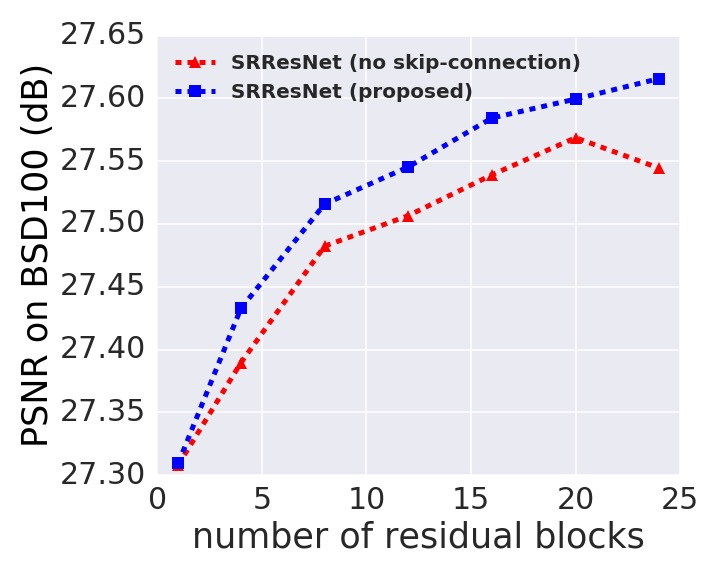
\includegraphics[width=0.5\textwidth]{images/used/appendix/jpg/psnr_vs_depth} &
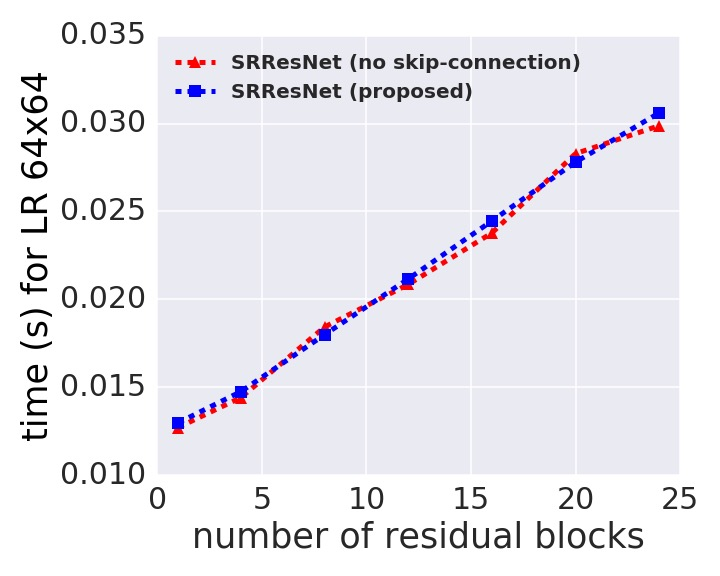
\includegraphics[width=0.5 \textwidth]{images/used/appendix/jpg/time_vs_depth}\\
\end{tabular}
\caption{Dependence of network performance (PSNR, time) on network depth. PSNR (left) calculated on BSD100. Time (right) averaged over 100 reconstructions of a random LR image with resolution 64$\times$64.}
\label{fig:app_psnrtime}
\end{figure*}

\clearpage
\subsection{Evolution of Generator during SRGAN training}
\label{app:evolution}
We further investigated how reconstructions of the \textbf{SRGAN} generator network evolve (visually) with increasing number of training iterations. Visual results obtained after different number of training iterations are illustrated in \figurename~\ref{fig:app_perceptual}. It is interesting that after only 20 thousand training iterations the generator substantially diverged from the SRResNet initialization and produces reconstruction with a lot of high frequency content, including noise. With increasing number of training iterations reconstructions of the \textit{baboon} from \textbf{Set14} appear closer to the reference image. However, there is visually little change during the last 50-100 thousand update iterations.
\begin{figure*}[ht!]
\begin{tabular}{ cx{3.7cm}cx{3.7cm}cx{3.7cm}cx{3.7cm}cx{3.7cm}}
~~~~~~~~~SRResNet & ~~~~~~20k & ~~~~~~~~~~~~~~40k & ~~~~~~~~~~~~~~~~~~60k & ~~~~~~~~~~~~~~~~~~~80k \\
\end{tabular}

\begin{tikzpicture}[zoomboxarray, zoomboxes below, zoomboxarray inner gap=0.1cm, zoomboxarray columns=2, zoomboxarray rows=2]
\node [image node] { 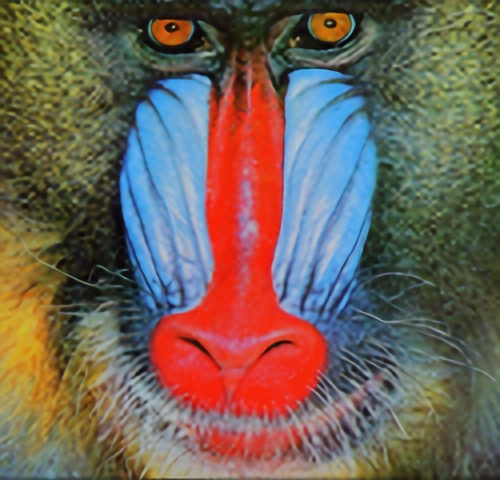
\includegraphics[trim=200 220 40 5, clip, width=1.3in]{images/used/appendix/jpg/evolution/baboon-net_gan_vgg54_16blocks_skip_fromMSE_noTV_noDS_evo_0} };
\zoombox[magnification=2,color code=red]{0.5,0.85}
\zoombox[magnification=2,color code=yellow]{0.7,0.55}
\zoombox[magnification=2,color code=orange]{0.35,0.3}
\zoombox[magnification=5,color code=lime]{0.86,0.25}
\end{tikzpicture}
\begin{tikzpicture}[zoomboxarray, zoomboxes below, zoomboxarray inner gap=0.1cm, zoomboxarray columns=2, zoomboxarray rows=2]
\node [image node] { 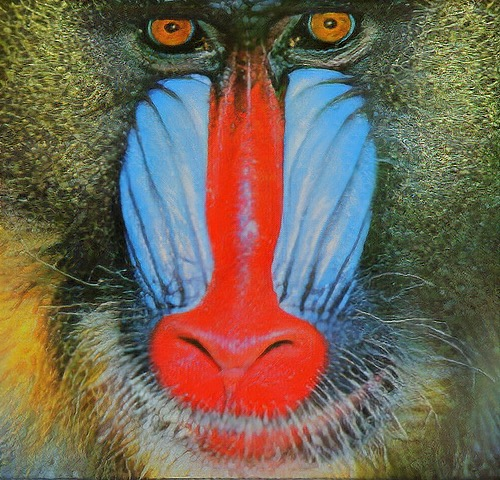
\includegraphics[trim=200 220 40 5, clip, width=1.3in]{images/used/appendix/jpg/evolution/baboon-net_gan_vgg54_16blocks_skip_fromMSE_noTV_noDS_evo_1} };
\zoombox[magnification=2,color code=red]{0.5,0.85}
\zoombox[magnification=2,color code=yellow]{0.7,0.55}
\zoombox[magnification=2,color code=orange]{0.35,0.3}
\zoombox[magnification=5,color code=lime]{0.86,0.25}
\end{tikzpicture}
\begin{tikzpicture}[zoomboxarray, zoomboxes below, zoomboxarray inner gap=0.1cm, zoomboxarray columns=2, zoomboxarray rows=2]
\node [image node] { 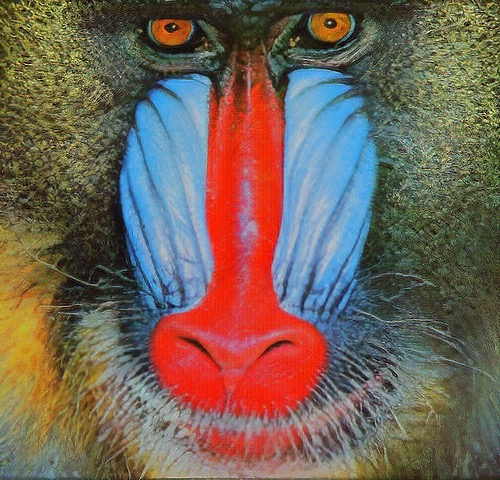
\includegraphics[trim=200 220 40 5, clip, width=1.3in]{images/used/appendix/jpg/evolution/baboon-net_gan_vgg54_16blocks_skip_fromMSE_noTV_noDS_evo_2} };
\zoombox[magnification=2,color code=red]{0.5,0.85}
\zoombox[magnification=2,color code=yellow]{0.7,0.55}
\zoombox[magnification=2,color code=orange]{0.35,0.3}
\zoombox[magnification=5,color code=lime]{0.86,0.25}
\end{tikzpicture}
\begin{tikzpicture}[zoomboxarray, zoomboxes below, zoomboxarray inner gap=0.1cm, zoomboxarray columns=2, zoomboxarray rows=2]
\node [image node] { 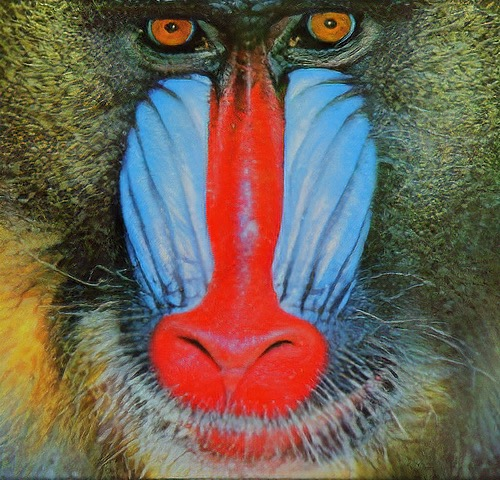
\includegraphics[trim=200 220 40 5, clip, width=1.3in]{images/used/appendix/jpg/evolution/baboon-net_gan_vgg54_16blocks_skip_fromMSE_noTV_noDS_evo_3} };
\zoombox[magnification=2,color code=red]{0.5,0.85}
\zoombox[magnification=2,color code=yellow]{0.7,0.55}
\zoombox[magnification=2,color code=orange]{0.35,0.3}
\zoombox[magnification=5,color code=lime]{0.86,0.25}
\end{tikzpicture}
\begin{tikzpicture}[zoomboxarray, zoomboxes below, zoomboxarray inner gap=0.1cm, zoomboxarray columns=2, zoomboxarray rows=2]
\node [image node] { 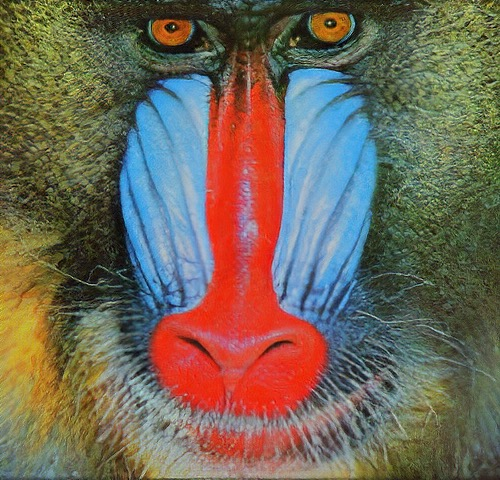
\includegraphics[trim=200 220 40 5, clip, width=1.3in]{images/used/appendix/jpg/evolution/baboon-net_gan_vgg54_16blocks_skip_fromMSE_noTV_noDS_evo_4} };
\zoombox[magnification=2,color code=red]{0.5,0.85}
\zoombox[magnification=2,color code=yellow]{0.7,0.55}
\zoombox[magnification=2,color code=orange]{0.35,0.3}
\zoombox[magnification=5,color code=lime]{0.86,0.25}
\end{tikzpicture}\\
\begin{tabular}{ cx{3.7cm}cx{3.7cm}cx{3.7cm}cx{3.7cm}cx{3.7cm}}
~~~~~~~~~~~~100k & ~~~~~~~~~~~~~~~~~140k & ~~~~~~~~~~~~~~~~~180k & ~~~~~~~~~~~~~~~~~~~SRGAN & ~~~~~~~~original HR image \\
\end{tabular}
\begin{tikzpicture}[zoomboxarray, zoomboxes below, zoomboxarray inner gap=0.1cm, zoomboxarray columns=2, zoomboxarray rows=2]
\node [image node] { 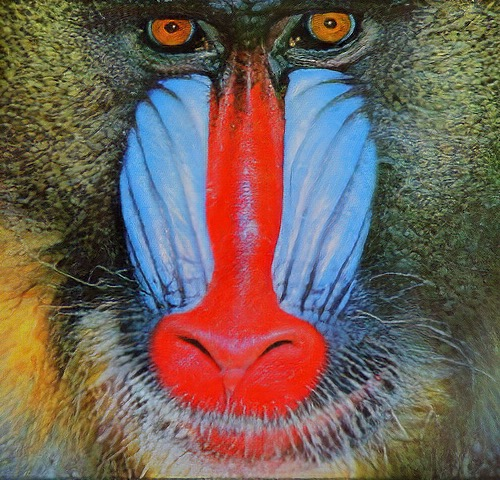
\includegraphics[trim=200 220 40 5, clip, width=1.3in]{images/used/appendix/jpg/evolution/baboon-net_gan_vgg54_16blocks_skip_fromMSE_noTV_noDS_evo_5} };
\zoombox[magnification=2,color code=red]{0.5,0.85}
\zoombox[magnification=2,color code=yellow]{0.7,0.55}
\zoombox[magnification=2,color code=orange]{0.35,0.3}
\zoombox[magnification=5,color code=lime]{0.86,0.25}
\end{tikzpicture}
\begin{tikzpicture}[zoomboxarray, zoomboxes below, zoomboxarray inner gap=0.1cm, zoomboxarray columns=2, zoomboxarray rows=2]
\node [image node] { 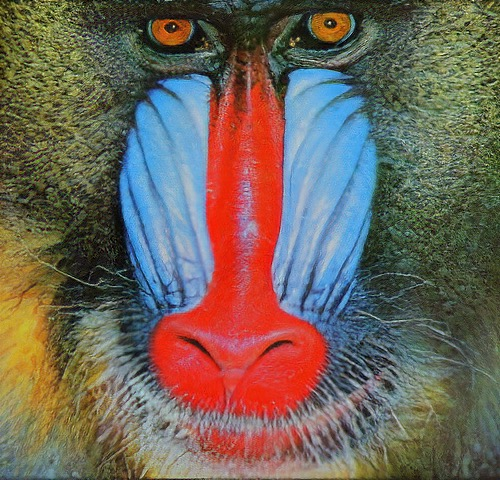
\includegraphics[trim=200 220 40 5, clip, width=1.3in]{images/used/appendix/jpg/evolution/baboon-net_gan_vgg54_16blocks_skip_fromMSE_noTV_noDS_evo_7} };
\zoombox[magnification=2,color code=red]{0.5,0.85}
\zoombox[magnification=2,color code=yellow]{0.7,0.55}
\zoombox[magnification=2,color code=orange]{0.35,0.3}
\zoombox[magnification=5,color code=lime]{0.86,0.25}
\end{tikzpicture}
\begin{tikzpicture}[zoomboxarray, zoomboxes below, zoomboxarray inner gap=0.1cm, zoomboxarray columns=2, zoomboxarray rows=2]
\node [image node] { 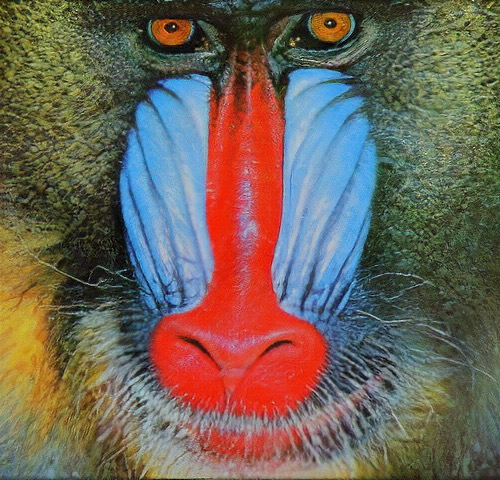
\includegraphics[trim=200 220 40 5, clip, width=1.3in]{images/used/appendix/jpg/evolution/baboon-net_gan_vgg54_16blocks_skip_fromMSE_noTV_noDS_evo_9} };
\zoombox[magnification=2,color code=red]{0.5,0.85}
\zoombox[magnification=2,color code=yellow]{0.7,0.55}
\zoombox[magnification=2,color code=orange]{0.35,0.3}
\zoombox[magnification=5,color code=lime]{0.86,0.25}
\end{tikzpicture}
\begin{tikzpicture}[zoomboxarray, zoomboxes below, zoomboxarray inner gap=0.1cm, zoomboxarray columns=2, zoomboxarray rows=2]
\node [image node] { 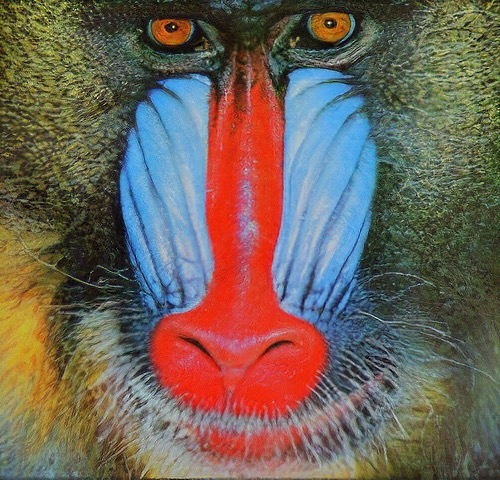
\includegraphics[trim=200 220 40 5, clip, width=1.3in]{images/used/appendix/jpg/evolution/baboon-net_gan_vgg54_16blocks_skip_fromMSE_noTV_noDS_final} };
\zoombox[magnification=2,color code=red]{0.5,0.85}
\zoombox[magnification=2,color code=yellow]{0.7,0.55}
\zoombox[magnification=2,color code=orange]{0.35,0.3}
\zoombox[magnification=5,color code=lime]{0.86,0.25}
\end{tikzpicture}
\begin{tikzpicture}[zoomboxarray, zoomboxes below, zoomboxarray inner gap=0.1cm, zoomboxarray columns=2, zoomboxarray rows=2]
\node [image node] { 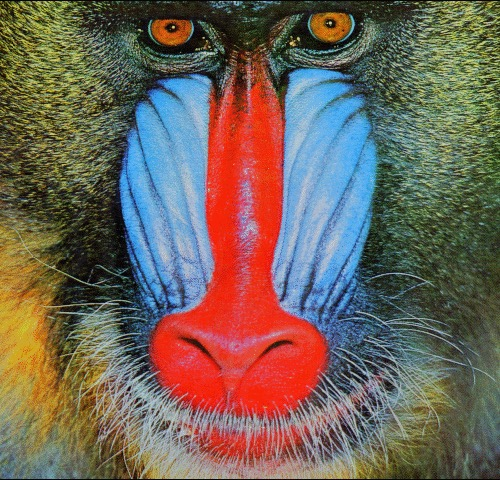
\includegraphics[trim=200 220 40 5, clip, width=1.3in]{images/used/jpg/baboon_HR} };
\zoombox[magnification=2,color code=red]{0.5,0.85}
\zoombox[magnification=2,color code=yellow]{0.7,0.55}
\zoombox[magnification=2,color code=orange]{0.35,0.3}
\zoombox[magnification=5,color code=lime]{0.86,0.25}
\end{tikzpicture}

\caption{Evolution of SRGAN generator network during training progress. Note: Generator initialized with SRResNet weights; learning rate set to  $10^{-4}$ for first 100k iterations, then reduced to $10^{-5}$ for another 100k iterations. [$4\times$ upscaling]}
\label{fig:app_perceptual}
\end{figure*}

\clearpage

\subsection{Mean opinion score (MOS) testing}
\label{app:MOS}

In all conducted \ac{MOS} tests we have asked 26 human raters to assign a score from 1 (Bad) to 5 (Excellent) to reconstructions of the $4\times$ downsampled versions of images from \textbf{Set5}, \textbf{Set14} and \textbf{BSD100}. On \textbf{BSD100} nine versions of each image were rated by each rater. On \textbf{Set5} and \textbf{Set14} the raters also rated three additional versions of the proposed methods to investigate different content losses. In total 26*100*9 + 26*14*12 + 26*5*12 = 29328 ratings were obtained, where each rater rated 1128 images. Images were presented in a completely randomized fashion without any indication of the employed super-resolution approach. The raters were calibrated on images not included in the testing set such that the nearest neighbor interpolated reconstruction should receive score 1 (Bad) and the original high-resolution image score 5 (Excellent).
The distribution of \ac{MOS} ratings on each individual data set is summarized in \figurename~\ref{fig:app_mosdist}. The average ordinal rank over all corresponding ratings of an image and rater are shown in \figurename~\ref{fig:app_mosrank}. Note that a score of 1 corresponds to the best rank and ranks are averaged for samples that would have the same ordinal ranking.
While results on \textbf{Set5} are somewhat inconclusive due to very small sample size and images with comparably little detail, ratings on \textbf{Set14} and especially on the large \textbf{BSD100} data set confirm that \textbf{SRGAN} is significantly better than any compared state-of-the-art method. In fact, \ac{MOS} ratings obtained with \textbf{SRGAN} are closer to those of the original high-resolution images than to those obtained with any reference method.
\begin{figure*}[h!]
\begin{tabular}{ccc}
Set5 & Set14 & BSD100 \\
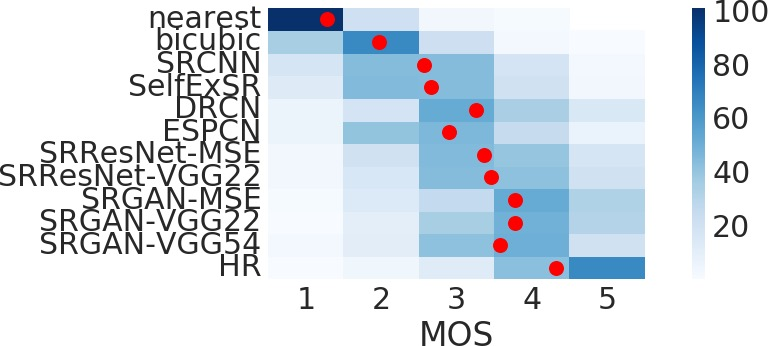
\includegraphics[width=0.3\textwidth]{images/used/appendix/jpg/MOS/MOS_heatmap_Set5_cropped}&
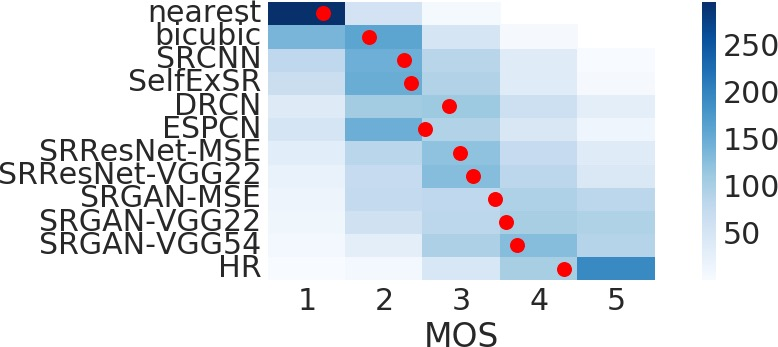
\includegraphics[width=0.3\textwidth]{images/used/appendix/jpg/MOS/MOS_heatmap_Set14_cropped} &
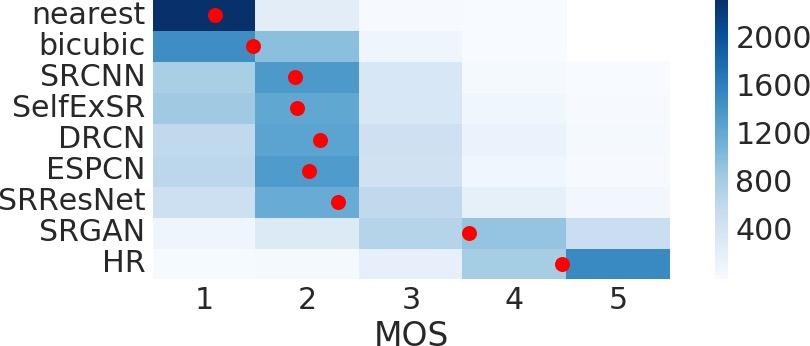
\includegraphics[width=0.3\textwidth]{images/used/appendix/jpg/MOS/MOS_heatmap_BSD100_cropped} \\
\end{tabular}
\caption{Color-coded distribution of MOS scores on Set5, Set14, BSD100. Mean shown as red marker, where the bins are centered around value i. [$4\times$ upscaling]}
\label{fig:app_mosdist}
\end{figure*}
\begin{figure*}[h!]
\begin{tabular}{ccc}
Set5 & Set14 & BSD100 \\
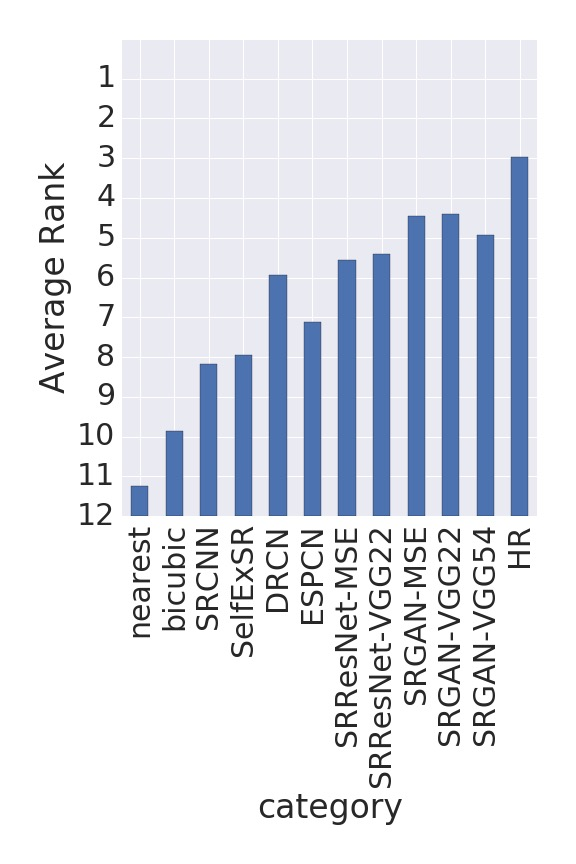
\includegraphics[width=0.3\textwidth]{images/used/appendix/jpg/MOS/Ranks_Set5}&
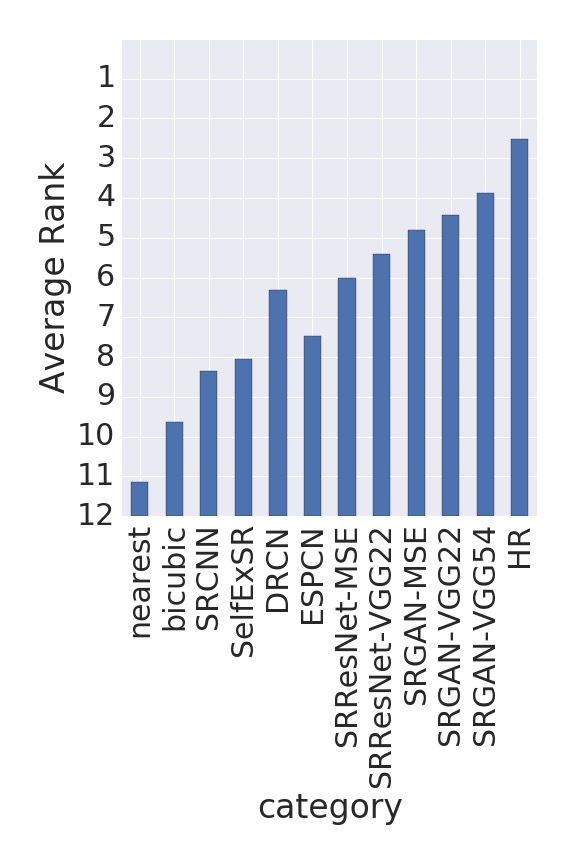
\includegraphics[width=0.3\textwidth]{images/used/appendix/jpg/MOS/Ranks_Set14} &
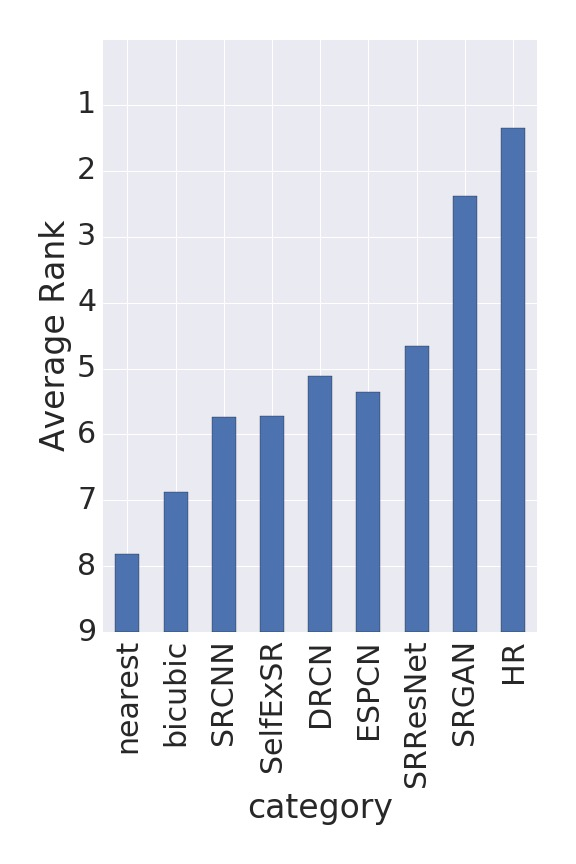
\includegraphics[width=0.3\textwidth]{images/used/appendix/jpg/MOS/Ranks_BSD100} \\
\end{tabular}
\caption{Average rank on Set5, Set14, BSD100 by averaging the ranks over all available individual ratings. [$4\times$ upscaling]}
\label{fig:app_mosrank}
\end{figure*}
\clearpage
\subsection{Set5 - Visual Results}
\label{app:Set5}
\begin{figure*}[h!]
\begin{tabular}{cccc}
bicubic & SRResNet & SRGAN & original \\
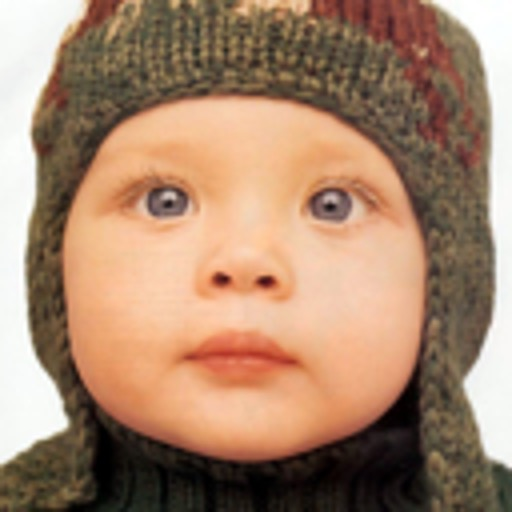
\includegraphics[width=1.4in]{images/used/appendix/jpg/Set5/baby_bicubic}&
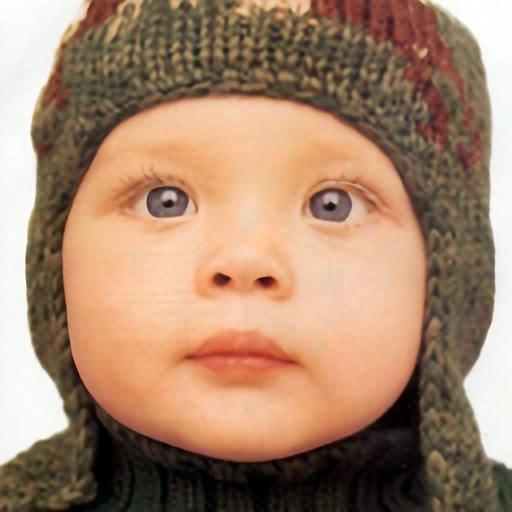
\includegraphics[width=1.4in]{images/used/appendix/jpg/Set5/baby_SRResNet-MSE} &
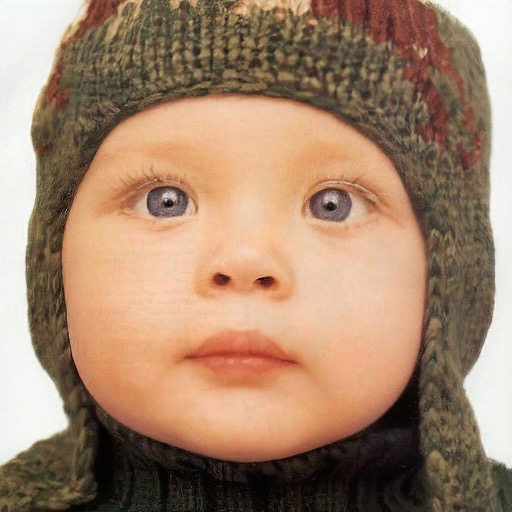
\includegraphics[width=1.4in]{images/used/appendix/jpg/Set5/baby_SRGAN-VGG54} &
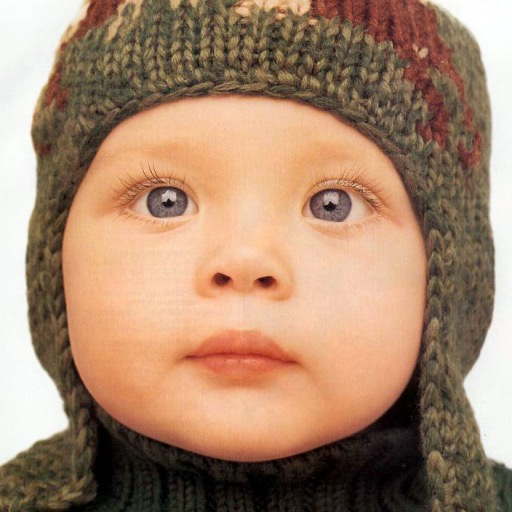
\includegraphics[width=1.4in]{images/used/appendix/jpg/Set5/baby_HR} \\
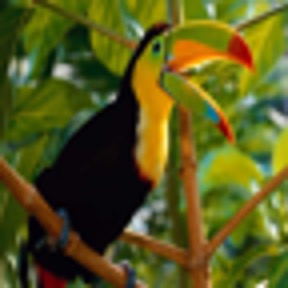
\includegraphics[width=1.4in]{images/used/appendix/jpg/Set5/bird_bicubic}&
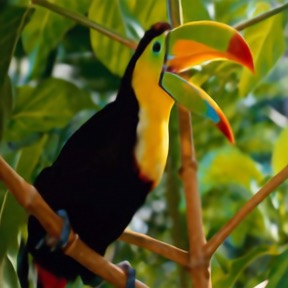
\includegraphics[width=1.4in]{images/used/appendix/jpg/Set5/bird_SRResNet-MSE} &
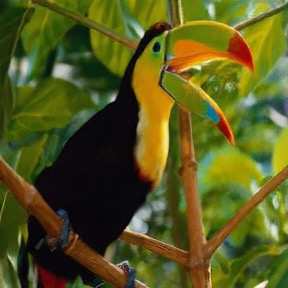
\includegraphics[width=1.4in]{images/used/appendix/jpg/Set5/bird_SRGAN-VGG54} &
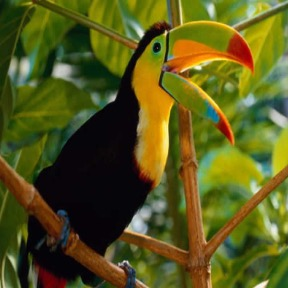
\includegraphics[width=1.4in]{images/used/appendix/jpg/Set5/bird_HR} \\
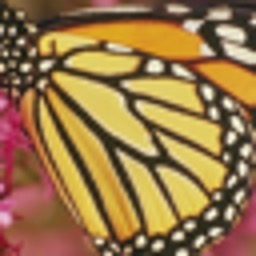
\includegraphics[width=1.4in]{images/used/appendix/jpg/Set5/butterfly_bicubic}&
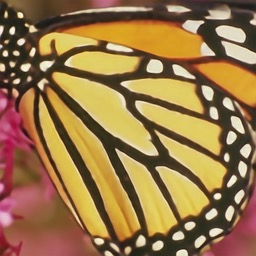
\includegraphics[width=1.4in]{images/used/appendix/jpg/Set5/butterfly_SRResNet-MSE} &
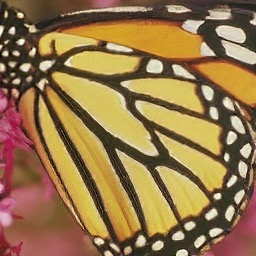
\includegraphics[width=1.4in]{images/used/appendix/jpg/Set5/butterfly_SRGAN-VGG54} &
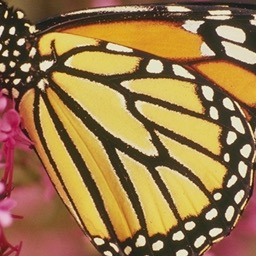
\includegraphics[width=1.4in]{images/used/appendix/jpg/Set5/butterfly_HR} \\
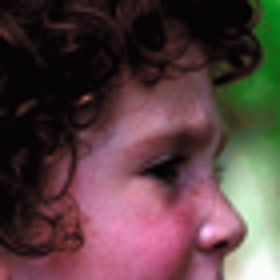
\includegraphics[width=1.4in]{images/used/appendix/jpg/Set5/head_bicubic}&
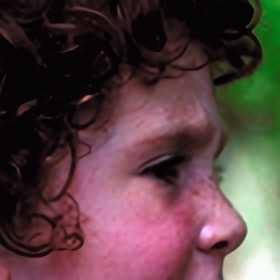
\includegraphics[width=1.4in]{images/used/appendix/jpg/Set5/head_SRResNet-MSE} &
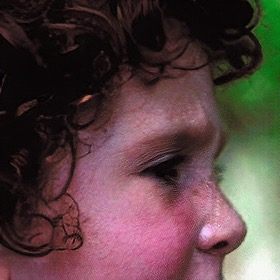
\includegraphics[width=1.4in]{images/used/appendix/jpg/Set5/head_SRGAN-VGG54} &
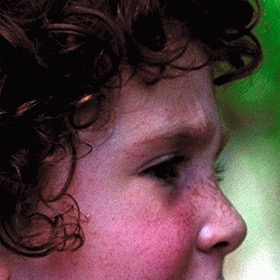
\includegraphics[width=1.4in]{images/used/appendix/jpg/Set5/head_HR} \\
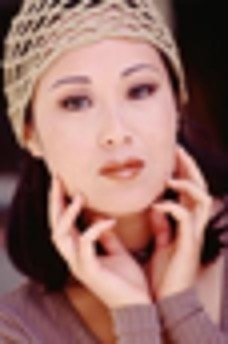
\includegraphics[width=1.4in]{images/used/appendix/jpg/Set5/woman_bicubic}&
\includegraphics[width=1.4in]{images/used/appendix/jpg/Set5/woman_SRResNet-MSE} &
\includegraphics[width=1.4in]{images/used/appendix/jpg/Set5/woman_SRGAN-VGG54} &
\includegraphics[width=1.4in]{images/used/appendix/jpg/Set5/woman_HR} \\
\end{tabular}
\label{fig:app_Set5}
\caption{Results for \textbf{Set5} using bicubic interpolation, SRResNet and SRGAN. [$4\times$ upscaling]}
\end{figure*}

\clearpage

\subsection{Set14 - Visual Results}
\label{app:Set14}
\begin{figure*}[h!]
\begin{tabular}{cccc}
bicubic & SRResNet & SRGAN & original \\
\includegraphics[width=1.5in]{images/used/appendix/jpg/Set14/baboon_bicubic}&
\includegraphics[width=1.5in]{images/used/appendix/jpg/Set14/baboon_SRResNet-MSE} &
\includegraphics[width=1.5in]{images/used/appendix/jpg/Set14/baboon_SRGAN-VGG54} &
\includegraphics[width=1.5in]{images/used/appendix/jpg/Set14/baboon_HR} \\
\includegraphics[width=1.5in]{images/used/appendix/jpg/Set14/barbara_bicubic}&
\includegraphics[width=1.5in]{images/used/appendix/jpg/Set14/barbara_SRResNet-MSE} &
\includegraphics[width=1.5in]{images/used/appendix/jpg/Set14/barbara_SRGAN-VGG54} &
\includegraphics[width=1.5in]{images/used/appendix/jpg/Set14/barbara_HR} \\
\includegraphics[width=1.5in]{images/used/appendix/jpg/Set14/bridge_bicubic}&
\includegraphics[width=1.5in]{images/used/appendix/jpg/Set14/bridge_SRResNet-MSE} &
\includegraphics[width=1.5in]{images/used/appendix/jpg/Set14/bridge_SRGAN-VGG54} &
\includegraphics[width=1.5in]{images/used/appendix/jpg/Set14/bridge_HR} \\
\includegraphics[width=1.5in]{images/used/appendix/jpg/Set14/coastguard_bicubic}&
\includegraphics[width=1.5in]{images/used/appendix/jpg/Set14/coastguard_SRResNet-MSE} &
\includegraphics[width=1.5in]{images/used/appendix/jpg/Set14/coastguard_SRGAN-VGG54} &
\includegraphics[width=1.5in]{images/used/appendix/jpg/Set14/coastguard_HR} \\
\includegraphics[width=1.5in]{images/used/appendix/jpg/Set14/comic_bicubic}&
\includegraphics[width=1.5in]{images/used/appendix/jpg/Set14/comic_SRResNet-MSE} &
\includegraphics[width=1.5in]{images/used/appendix/jpg/Set14/comic_SRGAN-VGG54} &
\includegraphics[width=1.5in]{images/used/appendix/jpg/Set14/comic_HR} \\
\end{tabular}
\label{fig:app_Set14a}
\caption{Results for \textbf{Set14} using bicubic interpolation, SRResNet and SRGAN. [$4\times$ upscaling]}
\end{figure*}

\begin{figure*}[h!]
\begin{tabular}{cccc}
bicubic & SRResNet & SRGAN & original \\
\includegraphics[width=1.5in]{images/used/appendix/jpg/Set14/face_bicubic}&
\includegraphics[width=1.5in]{images/used/appendix/jpg/Set14/face_SRResNet-MSE} &
\includegraphics[width=1.5in]{images/used/appendix/jpg/Set14/face_SRGAN-VGG54} &
\includegraphics[width=1.5in]{images/used/appendix/jpg/Set14/face_HR} \\
\includegraphics[width=1.5in]{images/used/appendix/jpg/Set14/flowers_bicubic}&
\includegraphics[width=1.5in]{images/used/appendix/jpg/Set14/flowers_SRResNet-MSE} &
\includegraphics[width=1.5in]{images/used/appendix/jpg/Set14/flowers_SRGAN-VGG54} &
\includegraphics[width=1.5in]{images/used/appendix/jpg/Set14/flowers_HR} \\
\includegraphics[width=1.5in]{images/used/appendix/jpg/Set14/foreman_bicubic}&
\includegraphics[width=1.5in]{images/used/appendix/jpg/Set14/foreman_SRResNet-MSE} &
\includegraphics[width=1.5in]{images/used/appendix/jpg/Set14/foreman_SRGAN-VGG54} &
\includegraphics[width=1.5in]{images/used/appendix/jpg/Set14/foreman_HR} \\
\includegraphics[width=1.5in]{images/used/appendix/jpg/Set14/lenna_bicubic}&
\includegraphics[width=1.5in]{images/used/appendix/jpg/Set14/lenna_SRResNet-MSE} &
\includegraphics[width=1.5in]{images/used/appendix/jpg/Set14/lenna_SRGAN-VGG54} &
\includegraphics[width=1.5in]{images/used/appendix/jpg/Set14/lenna_HR} \\
\includegraphics[width=1.5in]{images/used/appendix/jpg/Set14/man_bicubic}&
\includegraphics[width=1.5in]{images/used/appendix/jpg/Set14/man_SRResNet-MSE} &
\includegraphics[width=1.5in]{images/used/appendix/jpg/Set14/man_SRGAN-VGG54} &
\includegraphics[width=1.5in]{images/used/appendix/jpg/Set14/man_HR} \\
\end{tabular}
\label{fig:app_Set14b}
\caption{Results for \textbf{Set14} using bicubic interpolation , SRResNet and SRGAN. [$4\times$ upscaling]}
\end{figure*}

\begin{figure*}[h!]
\begin{tabular}{cccc}
bicubic & SRResNet & SRGAN & original \\
\includegraphics[width=1.5in]{images/used/appendix/jpg/Set14/monarch_bicubic}&
\includegraphics[width=1.5in]{images/used/appendix/jpg/Set14/monarch_SRResNet-MSE} &
\includegraphics[width=1.5in]{images/used/appendix/jpg/Set14/monarch_SRGAN-VGG54} &
\includegraphics[width=1.5in]{images/used/appendix/jpg/Set14/monarch_HR} \\
\includegraphics[width=1.5in]{images/used/appendix/jpg/Set14/pepper_bicubic}&
\includegraphics[width=1.5in]{images/used/appendix/jpg/Set14/pepper_SRResNet-MSE} &
\includegraphics[width=1.5in]{images/used/appendix/jpg/Set14/pepper_SRGAN-VGG54} &
\includegraphics[width=1.5in]{images/used/appendix/jpg/Set14/pepper_HR} \\
\includegraphics[width=1.5in]{images/used/appendix/jpg/Set14/ppt3_bicubic}&
\includegraphics[width=1.5in]{images/used/appendix/jpg/Set14/ppt3_SRResNet-MSE} &
\includegraphics[width=1.5in]{images/used/appendix/jpg/Set14/ppt3_SRGAN-VGG54} &
\includegraphics[width=1.5in]{images/used/appendix/jpg/Set14/ppt3_HR} \\
\includegraphics[width=1.5in]{images/used/appendix/jpg/Set14/zebra_bicubic}&
\includegraphics[width=1.5in]{images/used/appendix/jpg/Set14/zebra_SRResNet-MSE} &
\includegraphics[width=1.5in]{images/used/appendix/jpg/Set14/zebra_SRGAN-VGG54} &
\includegraphics[width=1.5in]{images/used/appendix/jpg/Set14/zebra_HR} \\
\end{tabular}
\label{fig:app_Set14c}
\caption{Results for \textbf{Set14} using bicubic interpolation, SRResNet and SRGAN. [$4\times$ upscaling]}
\end{figure*}
\clearpage
\subsection{BSD100 (five random samples) - Visual Results}
\label{app:BSD100}
\begin{figure*}[h!]
\begin{tabular}{cccc}
bicubic & SRResNet & SRGAN & original \\
\includegraphics[width=1.5in]{images/used/appendix/jpg/BSD100/219090_bicubic}&
\includegraphics[width=1.5in]{images/used/appendix/jpg/BSD100/219090_SRResNet-MSE} &
\includegraphics[width=1.5in]{images/used/appendix/jpg/BSD100/219090_SRGAN-VGG54} &
\includegraphics[width=1.5in]{images/used/appendix/jpg/BSD100/219090_HR} \\
\includegraphics[width=1.5in]{images/used/appendix/jpg/BSD100/45096_bicubic}&
\includegraphics[width=1.5in]{images/used/appendix/jpg/BSD100/45096_SRResNet-MSE} &
\includegraphics[width=1.5in]{images/used/appendix/jpg/BSD100/45096_SRGAN-VGG54} &
\includegraphics[width=1.5in]{images/used/appendix/jpg/BSD100/45096_HR} \\
\includegraphics[width=1.5in]{images/used/appendix/jpg/BSD100/196073_bicubic}&
\includegraphics[width=1.5in]{images/used/appendix/jpg/BSD100/196073_SRResNet-MSE} &
\includegraphics[width=1.5in]{images/used/appendix/jpg/BSD100/196073_SRGAN-VGG54} &
\includegraphics[width=1.5in]{images/used/appendix/jpg/BSD100/196073_HR} \\
\includegraphics[width=1.5in]{images/used/appendix/jpg/BSD100/54082_bicubic}&
\includegraphics[width=1.5in]{images/used/appendix/jpg/BSD100/54082_SRResNet-MSE} &
\includegraphics[width=1.5in]{images/used/appendix/jpg/BSD100/54082_SRGAN-VGG54} &
\includegraphics[width=1.5in]{images/used/appendix/jpg/BSD100/54082_HR} \\
\includegraphics[width=1.5in]{images/used/appendix/jpg/BSD100/220075_bicubic}&
\includegraphics[width=1.5in]{images/used/appendix/jpg/BSD100/220075_SRResNet-MSE} &
\includegraphics[width=1.5in]{images/used/appendix/jpg/BSD100/220075_SRGAN-VGG54} &
\includegraphics[width=1.5in]{images/used/appendix/jpg/BSD100/220075_HR} \\
\end{tabular}
\label{fig:app_BSD100}
\caption{Results for five random samples of \textbf{BSD100} using bicubic interpolation, SRResNet and SRGAN. [$4\times$ upscaling]}
\end{figure*}

\end{document}


